% Options for packages loaded elsewhere
\PassOptionsToPackage{unicode}{hyperref}
\PassOptionsToPackage{hyphens}{url}
%
\documentclass[
]{article}
\usepackage{amsmath,amssymb}
\usepackage{lmodern}
\usepackage{ifxetex,ifluatex}
\ifnum 0\ifxetex 1\fi\ifluatex 1\fi=0 % if pdftex
  \usepackage[T1]{fontenc}
  \usepackage[utf8]{inputenc}
  \usepackage{textcomp} % provide euro and other symbols
\else % if luatex or xetex
  \usepackage{unicode-math}
  \defaultfontfeatures{Scale=MatchLowercase}
  \defaultfontfeatures[\rmfamily]{Ligatures=TeX,Scale=1}
\fi
% Use upquote if available, for straight quotes in verbatim environments
\IfFileExists{upquote.sty}{\usepackage{upquote}}{}
\IfFileExists{microtype.sty}{% use microtype if available
  \usepackage[]{microtype}
  \UseMicrotypeSet[protrusion]{basicmath} % disable protrusion for tt fonts
}{}
\makeatletter
\@ifundefined{KOMAClassName}{% if non-KOMA class
  \IfFileExists{parskip.sty}{%
    \usepackage{parskip}
  }{% else
    \setlength{\parindent}{0pt}
    \setlength{\parskip}{6pt plus 2pt minus 1pt}}
}{% if KOMA class
  \KOMAoptions{parskip=half}}
\makeatother
\usepackage{xcolor}
\IfFileExists{xurl.sty}{\usepackage{xurl}}{} % add URL line breaks if available
\IfFileExists{bookmark.sty}{\usepackage{bookmark}}{\usepackage{hyperref}}
\hypersetup{
  pdftitle={R Notebook},
  hidelinks,
  pdfcreator={LaTeX via pandoc}}
\urlstyle{same} % disable monospaced font for URLs
\usepackage[margin=1in]{geometry}
\usepackage{color}
\usepackage{fancyvrb}
\newcommand{\VerbBar}{|}
\newcommand{\VERB}{\Verb[commandchars=\\\{\}]}
\DefineVerbatimEnvironment{Highlighting}{Verbatim}{commandchars=\\\{\}}
% Add ',fontsize=\small' for more characters per line
\usepackage{framed}
\definecolor{shadecolor}{RGB}{248,248,248}
\newenvironment{Shaded}{\begin{snugshade}}{\end{snugshade}}
\newcommand{\AlertTok}[1]{\textcolor[rgb]{0.94,0.16,0.16}{#1}}
\newcommand{\AnnotationTok}[1]{\textcolor[rgb]{0.56,0.35,0.01}{\textbf{\textit{#1}}}}
\newcommand{\AttributeTok}[1]{\textcolor[rgb]{0.77,0.63,0.00}{#1}}
\newcommand{\BaseNTok}[1]{\textcolor[rgb]{0.00,0.00,0.81}{#1}}
\newcommand{\BuiltInTok}[1]{#1}
\newcommand{\CharTok}[1]{\textcolor[rgb]{0.31,0.60,0.02}{#1}}
\newcommand{\CommentTok}[1]{\textcolor[rgb]{0.56,0.35,0.01}{\textit{#1}}}
\newcommand{\CommentVarTok}[1]{\textcolor[rgb]{0.56,0.35,0.01}{\textbf{\textit{#1}}}}
\newcommand{\ConstantTok}[1]{\textcolor[rgb]{0.00,0.00,0.00}{#1}}
\newcommand{\ControlFlowTok}[1]{\textcolor[rgb]{0.13,0.29,0.53}{\textbf{#1}}}
\newcommand{\DataTypeTok}[1]{\textcolor[rgb]{0.13,0.29,0.53}{#1}}
\newcommand{\DecValTok}[1]{\textcolor[rgb]{0.00,0.00,0.81}{#1}}
\newcommand{\DocumentationTok}[1]{\textcolor[rgb]{0.56,0.35,0.01}{\textbf{\textit{#1}}}}
\newcommand{\ErrorTok}[1]{\textcolor[rgb]{0.64,0.00,0.00}{\textbf{#1}}}
\newcommand{\ExtensionTok}[1]{#1}
\newcommand{\FloatTok}[1]{\textcolor[rgb]{0.00,0.00,0.81}{#1}}
\newcommand{\FunctionTok}[1]{\textcolor[rgb]{0.00,0.00,0.00}{#1}}
\newcommand{\ImportTok}[1]{#1}
\newcommand{\InformationTok}[1]{\textcolor[rgb]{0.56,0.35,0.01}{\textbf{\textit{#1}}}}
\newcommand{\KeywordTok}[1]{\textcolor[rgb]{0.13,0.29,0.53}{\textbf{#1}}}
\newcommand{\NormalTok}[1]{#1}
\newcommand{\OperatorTok}[1]{\textcolor[rgb]{0.81,0.36,0.00}{\textbf{#1}}}
\newcommand{\OtherTok}[1]{\textcolor[rgb]{0.56,0.35,0.01}{#1}}
\newcommand{\PreprocessorTok}[1]{\textcolor[rgb]{0.56,0.35,0.01}{\textit{#1}}}
\newcommand{\RegionMarkerTok}[1]{#1}
\newcommand{\SpecialCharTok}[1]{\textcolor[rgb]{0.00,0.00,0.00}{#1}}
\newcommand{\SpecialStringTok}[1]{\textcolor[rgb]{0.31,0.60,0.02}{#1}}
\newcommand{\StringTok}[1]{\textcolor[rgb]{0.31,0.60,0.02}{#1}}
\newcommand{\VariableTok}[1]{\textcolor[rgb]{0.00,0.00,0.00}{#1}}
\newcommand{\VerbatimStringTok}[1]{\textcolor[rgb]{0.31,0.60,0.02}{#1}}
\newcommand{\WarningTok}[1]{\textcolor[rgb]{0.56,0.35,0.01}{\textbf{\textit{#1}}}}
\usepackage{graphicx}
\makeatletter
\def\maxwidth{\ifdim\Gin@nat@width>\linewidth\linewidth\else\Gin@nat@width\fi}
\def\maxheight{\ifdim\Gin@nat@height>\textheight\textheight\else\Gin@nat@height\fi}
\makeatother
% Scale images if necessary, so that they will not overflow the page
% margins by default, and it is still possible to overwrite the defaults
% using explicit options in \includegraphics[width, height, ...]{}
\setkeys{Gin}{width=\maxwidth,height=\maxheight,keepaspectratio}
% Set default figure placement to htbp
\makeatletter
\def\fps@figure{htbp}
\makeatother
\setlength{\emergencystretch}{3em} % prevent overfull lines
\providecommand{\tightlist}{%
  \setlength{\itemsep}{0pt}\setlength{\parskip}{0pt}}
\setcounter{secnumdepth}{-\maxdimen} % remove section numbering
\ifluatex
  \usepackage{selnolig}  % disable illegal ligatures
\fi

\title{R Notebook}
\author{}
\date{\vspace{-2.5em}}

\begin{document}
\maketitle

\begin{Shaded}
\begin{Highlighting}[]
\FunctionTok{library}\NormalTok{(tidyverse)}
\end{Highlighting}
\end{Shaded}

\begin{verbatim}
## Warning in system("timedatectl", intern = TRUE): running command 'timedatectl'
## had status 1
\end{verbatim}

\begin{verbatim}
## -- Attaching packages --------------------------------------- tidyverse 1.3.1 --
\end{verbatim}

\begin{verbatim}
## v ggplot2 3.3.5     v purrr   0.3.4
## v tibble  3.1.4     v dplyr   1.0.7
## v tidyr   1.1.4     v stringr 1.4.0
## v readr   2.0.1     v forcats 0.5.1
\end{verbatim}

\begin{verbatim}
## -- Conflicts ------------------------------------------ tidyverse_conflicts() --
## x dplyr::filter() masks stats::filter()
## x dplyr::lag()    masks stats::lag()
\end{verbatim}

\begin{Shaded}
\begin{Highlighting}[]
\NormalTok{all\_counts }\OtherTok{\textless{}{-}} \FunctionTok{readRDS}\NormalTok{(}\AttributeTok{file=} \StringTok{"Data/pc\_count\_matrix.rds"}\NormalTok{)}
\NormalTok{avg\_counts }\OtherTok{\textless{}{-}} \FunctionTok{readRDS}\NormalTok{(}\AttributeTok{file=}\StringTok{"Data/avg\_pc\_count\_matrix.rds"}\NormalTok{)}
\NormalTok{diff\_counts }\OtherTok{\textless{}{-}} \FunctionTok{readRDS}\NormalTok{(}\AttributeTok{file=}\StringTok{"Data/diff\_pc\_count\_matrix.rds"}\NormalTok{)}
\NormalTok{meta }\OtherTok{\textless{}{-}} \FunctionTok{suppressMessages}\NormalTok{(readr}\SpecialCharTok{::}\FunctionTok{read\_tsv}\NormalTok{(}\StringTok{"Data/complete\_meta\_data.tsv"}\NormalTok{))}
\NormalTok{tissue\_types }\OtherTok{\textless{}{-}} \FunctionTok{unique}\NormalTok{(meta }\SpecialCharTok{\%\textgreater{}\%} \FunctionTok{pull}\NormalTok{(tissue\_type))}
\NormalTok{TFs}\OtherTok{\textless{}{-}} \FunctionTok{c}\NormalTok{(}\StringTok{"Ascl1"}\NormalTok{, }\StringTok{"Hes1"}\NormalTok{, }\StringTok{"Neurod1"}\NormalTok{, }\StringTok{"Mecp2"}\NormalTok{, }\StringTok{"Mef2c"}\NormalTok{, }\StringTok{"Runx1"}\NormalTok{, }\StringTok{"Tcf4"}\NormalTok{, }\StringTok{"Pax6"}\NormalTok{)}
\end{Highlighting}
\end{Shaded}

Investigate the most highly expressed gene (sum of all stages) for each
tissue type

\begin{Shaded}
\begin{Highlighting}[]
\NormalTok{maxes\_list }\OtherTok{\textless{}{-}} \FunctionTok{list}\NormalTok{()}
\ControlFlowTok{for}\NormalTok{ (tissue }\ControlFlowTok{in}\NormalTok{ tissue\_types)\{}
\NormalTok{  tissue\_subset\_ids }\OtherTok{\textless{}{-}}\NormalTok{ meta }\SpecialCharTok{\%\textgreater{}\%} \FunctionTok{filter}\NormalTok{(tissue\_type }\SpecialCharTok{==}\NormalTok{ tissue) }\SpecialCharTok{\%\textgreater{}\%} \FunctionTok{pull}\NormalTok{(id)}
\NormalTok{  all\_sums }\OtherTok{\textless{}{-}} \FunctionTok{apply}\NormalTok{(all\_counts[,tissue\_subset\_ids],}\DecValTok{1}\NormalTok{, sum)}
\NormalTok{  maxes\_list[tissue] }\OtherTok{\textless{}{-}} \FunctionTok{names}\NormalTok{(all\_sums)[}\FunctionTok{which.max}\NormalTok{(all\_sums)]}
\NormalTok{\}}
\ControlFlowTok{for}\NormalTok{ (name }\ControlFlowTok{in} \FunctionTok{names}\NormalTok{(maxes\_list))\{}
  \FunctionTok{print}\NormalTok{(}\FunctionTok{paste0}\NormalTok{(}\StringTok{"The most highly expressed protein in "}\NormalTok{, name, }\StringTok{" : "}\NormalTok{, maxes\_list[name]))}
\NormalTok{\}}
\end{Highlighting}
\end{Shaded}

\begin{verbatim}
## [1] "The most highly expressed protein in forebrain : Tuba1a"
## [1] "The most highly expressed protein in midbrain : Tuba1a"
## [1] "The most highly expressed protein in hindbrain : Tuba1a"
## [1] "The most highly expressed protein in embryonic facial prominence : Hba-a2"
## [1] "The most highly expressed protein in heart : Hba-a2"
## [1] "The most highly expressed protein in limb : Hba-a2"
## [1] "The most highly expressed protein in liver : Hba-a2"
## [1] "The most highly expressed protein in neural tube : Tuba1a"
## [1] "The most highly expressed protein in lung : Sftpc"
## [1] "The most highly expressed protein in stomach : Cym"
## [1] "The most highly expressed protein in intestine : mt-Atp6"
## [1] "The most highly expressed protein in kidney : mt-Atp6"
## [1] "The most highly expressed protein in thymus : Actb"
## [1] "The most highly expressed protein in skeletal muscle tissue : Acta1"
## [1] "The most highly expressed protein in spleen : Hba-a2"
## [1] "The most highly expressed protein in urinary bladder : Actg2"
## [1] "The most highly expressed protein in adrenal gland : mt-Atp6"
\end{verbatim}

Same thing as above but excluding the mitochondria

\begin{Shaded}
\begin{Highlighting}[]
\NormalTok{maxes\_list }\OtherTok{\textless{}{-}} \FunctionTok{list}\NormalTok{()}
\ControlFlowTok{for}\NormalTok{ (tissue }\ControlFlowTok{in}\NormalTok{ tissue\_types)\{}
\NormalTok{  tissue\_subset\_ids }\OtherTok{\textless{}{-}}\NormalTok{ meta }\SpecialCharTok{\%\textgreater{}\%} \FunctionTok{filter}\NormalTok{(tissue\_type }\SpecialCharTok{==}\NormalTok{ tissue) }\SpecialCharTok{\%\textgreater{}\%} \FunctionTok{pull}\NormalTok{(id)}
\NormalTok{  all\_sums }\OtherTok{\textless{}{-}} \FunctionTok{apply}\NormalTok{(all\_counts[,tissue\_subset\_ids],}\DecValTok{1}\NormalTok{, sum)}
\NormalTok{  all\_sums }\OtherTok{\textless{}{-}}\NormalTok{ all\_sums[}\SpecialCharTok{!}\FunctionTok{sapply}\NormalTok{(}\FunctionTok{names}\NormalTok{(all\_sums), startsWith, }\StringTok{"mt{-}"}\NormalTok{)]}
\NormalTok{  maxes\_list[tissue] }\OtherTok{\textless{}{-}} \FunctionTok{names}\NormalTok{(all\_sums)[}\FunctionTok{which.max}\NormalTok{(all\_sums)]}
\NormalTok{\}}
\ControlFlowTok{for}\NormalTok{ (name }\ControlFlowTok{in} \FunctionTok{names}\NormalTok{(maxes\_list))\{}
  \FunctionTok{print}\NormalTok{(}\FunctionTok{paste0}\NormalTok{(}\StringTok{"The most highly expressed protein in "}\NormalTok{, name, }\StringTok{" : "}\NormalTok{, maxes\_list[name]))}
\NormalTok{\}}
\end{Highlighting}
\end{Shaded}

\begin{verbatim}
## [1] "The most highly expressed protein in forebrain : Tuba1a"
## [1] "The most highly expressed protein in midbrain : Tuba1a"
## [1] "The most highly expressed protein in hindbrain : Tuba1a"
## [1] "The most highly expressed protein in embryonic facial prominence : Hba-a2"
## [1] "The most highly expressed protein in heart : Hba-a2"
## [1] "The most highly expressed protein in limb : Hba-a2"
## [1] "The most highly expressed protein in liver : Hba-a2"
## [1] "The most highly expressed protein in neural tube : Tuba1a"
## [1] "The most highly expressed protein in lung : Sftpc"
## [1] "The most highly expressed protein in stomach : Cym"
## [1] "The most highly expressed protein in intestine : Apoa1"
## [1] "The most highly expressed protein in kidney : Hba-a2"
## [1] "The most highly expressed protein in thymus : Actb"
## [1] "The most highly expressed protein in skeletal muscle tissue : Acta1"
## [1] "The most highly expressed protein in spleen : Hba-a2"
## [1] "The most highly expressed protein in urinary bladder : Actg2"
## [1] "The most highly expressed protein in adrenal gland : Hba-a2"
\end{verbatim}

Top 5 Universally highly expressed protein across all tissues regardless
of stages (without processing)

\begin{Shaded}
\begin{Highlighting}[]
\DocumentationTok{\#\#Collapse dev\_stages}
\NormalTok{collapsed\_matrices }\OtherTok{\textless{}{-}} \FunctionTok{matrix}\NormalTok{(}\AttributeTok{data=}\ConstantTok{NA}\NormalTok{, }\AttributeTok{nrow =} \FunctionTok{nrow}\NormalTok{(all\_counts), }\AttributeTok{ncol =} \FunctionTok{length}\NormalTok{(tissue\_types))}
\FunctionTok{rownames}\NormalTok{(collapsed\_matrices) }\OtherTok{\textless{}{-}} \FunctionTok{rownames}\NormalTok{(all\_counts)}
\NormalTok{walker }\OtherTok{\textless{}{-}} \DecValTok{1}
\ControlFlowTok{for}\NormalTok{ (tissue }\ControlFlowTok{in}\NormalTok{ tissue\_types)\{}
\NormalTok{  tissue\_subset\_ids }\OtherTok{\textless{}{-}}\NormalTok{ meta }\SpecialCharTok{\%\textgreater{}\%} \FunctionTok{filter}\NormalTok{(tissue\_type }\SpecialCharTok{==}\NormalTok{ tissue) }\SpecialCharTok{\%\textgreater{}\%} \FunctionTok{pull}\NormalTok{(id)}
\NormalTok{  all\_avgs }\OtherTok{\textless{}{-}} \FunctionTok{apply}\NormalTok{(all\_counts[,tissue\_subset\_ids],}\DecValTok{1}\NormalTok{, mean)}
\NormalTok{  collapsed\_matrices[,walker] }\OtherTok{\textless{}{-}}\NormalTok{ all\_avgs}
\NormalTok{  walker }\OtherTok{\textless{}{-}}\NormalTok{ walker }\SpecialCharTok{+} \DecValTok{1}
\NormalTok{\}}
\NormalTok{all\_sums }\OtherTok{\textless{}{-}} \FunctionTok{apply}\NormalTok{(collapsed\_matrices,}\DecValTok{1}\NormalTok{, sum)}
\ControlFlowTok{for}\NormalTok{ (i }\ControlFlowTok{in} \DecValTok{1}\SpecialCharTok{:}\DecValTok{10}\NormalTok{)\{}
  \FunctionTok{print}\NormalTok{(}\FunctionTok{paste0}\NormalTok{(}\StringTok{"The highests expressed protein acrossed all tissue in order "}\NormalTok{,i ,}\StringTok{": "}\NormalTok{, }\FunctionTok{names}\NormalTok{(}\FunctionTok{sort}\NormalTok{(all\_sums,}\AttributeTok{decreasing=}\ConstantTok{TRUE}\NormalTok{))[i]))}
\NormalTok{\}}
\end{Highlighting}
\end{Shaded}

\begin{verbatim}
## [1] "The highests expressed protein acrossed all tissue in order 1: Hba-a2"
## [1] "The highests expressed protein acrossed all tissue in order 2: Hbb-bs"
## [1] "The highests expressed protein acrossed all tissue in order 3: mt-Atp6"
## [1] "The highests expressed protein acrossed all tissue in order 4: Hba-a1"
## [1] "The highests expressed protein acrossed all tissue in order 5: Hbb-bt"
## [1] "The highests expressed protein acrossed all tissue in order 6: mt-Atp8"
## [1] "The highests expressed protein acrossed all tissue in order 7: Actb"
## [1] "The highests expressed protein acrossed all tissue in order 8: Ftl1"
## [1] "The highests expressed protein acrossed all tissue in order 9: Ppia"
## [1] "The highests expressed protein acrossed all tissue in order 10: Acta1"
\end{verbatim}

Expression profile of the highest expressed protein across all tissues
Hba-a2 Extract only Hba-a2 information

\begin{Shaded}
\begin{Highlighting}[]
\FunctionTok{library}\NormalTok{(ggplot2)}
\NormalTok{target\_protein }\OtherTok{\textless{}{-}} \StringTok{"Hba{-}a2"}
\NormalTok{unique\_dev\_stages }\OtherTok{\textless{}{-}} \FunctionTok{unique}\NormalTok{(meta }\SpecialCharTok{\%\textgreater{}\%} \FunctionTok{pull}\NormalTok{(dev\_stage))}
\NormalTok{Hba\_matrix }\OtherTok{\textless{}{-}} \FunctionTok{matrix}\NormalTok{(}\AttributeTok{data=}\ConstantTok{NA}\NormalTok{, }\AttributeTok{nrow=}\FunctionTok{length}\NormalTok{(tissue\_types), }\AttributeTok{ncol=}\DecValTok{3}\NormalTok{)}
\FunctionTok{colnames}\NormalTok{(Hba\_matrix) }\OtherTok{\textless{}{-}} \FunctionTok{c}\NormalTok{(}\StringTok{"count"}\NormalTok{, }\StringTok{"dev\_stage"}\NormalTok{, }\StringTok{"tissue\_type"}\NormalTok{)}
\NormalTok{Hba\_frame }\OtherTok{\textless{}{-}} \FunctionTok{data.frame}\NormalTok{(Hba\_matrix)}
\NormalTok{walker }\OtherTok{\textless{}{-}} \DecValTok{1}
\ControlFlowTok{for}\NormalTok{ (exp\_id }\ControlFlowTok{in} \FunctionTok{names}\NormalTok{(avg\_counts[target\_protein,]))\{}
\NormalTok{    Hba\_frame[walker, }\StringTok{"count"}\NormalTok{] }\OtherTok{\textless{}{-}}\NormalTok{ avg\_counts[target\_protein, exp\_id]}
\NormalTok{    Hba\_frame[walker, }\StringTok{"dev\_stage"}\NormalTok{] }\OtherTok{\textless{}{-}}\NormalTok{ meta }\SpecialCharTok{\%\textgreater{}\%} \FunctionTok{filter}\NormalTok{(id}\SpecialCharTok{==}\NormalTok{exp\_id) }\SpecialCharTok{\%\textgreater{}\%} \FunctionTok{pull}\NormalTok{(dev\_stage)}
\NormalTok{    Hba\_frame[walker, }\StringTok{"tissue\_type"}\NormalTok{] }\OtherTok{\textless{}{-}}\NormalTok{ meta }\SpecialCharTok{\%\textgreater{}\%} \FunctionTok{filter}\NormalTok{(id}\SpecialCharTok{==}\NormalTok{exp\_id) }\SpecialCharTok{\%\textgreater{}\%} \FunctionTok{pull}\NormalTok{(tissue\_type)}
\NormalTok{    walker }\OtherTok{\textless{}{-}}\NormalTok{ walker }\SpecialCharTok{+} \DecValTok{1}
\NormalTok{\}}
\NormalTok{Hba\_frame}\SpecialCharTok{$}\NormalTok{count }\OtherTok{\textless{}{-}} \FunctionTok{log2}\NormalTok{(Hba\_frame}\SpecialCharTok{$}\NormalTok{count) }
\end{Highlighting}
\end{Shaded}

Plot the extracted information

\begin{Shaded}
\begin{Highlighting}[]
\FunctionTok{library}\NormalTok{(ggrepel)}
\NormalTok{make\_label }\OtherTok{\textless{}{-}} \ControlFlowTok{function}\NormalTok{(row)\{}
  \ControlFlowTok{if}\NormalTok{ (row[}\StringTok{\textquotesingle{}dev\_stage\textquotesingle{}}\NormalTok{] }\SpecialCharTok{==} \FunctionTok{max}\NormalTok{(Hba\_frame }\SpecialCharTok{\%\textgreater{}\%} \FunctionTok{filter}\NormalTok{(tissue\_type}\SpecialCharTok{==}\NormalTok{row[}\StringTok{\textquotesingle{}tissue\_type\textquotesingle{}}\NormalTok{]) }\SpecialCharTok{\%\textgreater{}\%} \FunctionTok{pull}\NormalTok{(dev\_stage)))\{}
    \CommentTok{\#print(max(Hba\_frame \%\textgreater{}\% filter(tissue\_type==tissue) \%\textgreater{}\% pull(dev\_stage)))\textbackslash{}}
     \FunctionTok{return}\NormalTok{(}\FunctionTok{as.character}\NormalTok{(row[}\StringTok{\textquotesingle{}tissue\_type\textquotesingle{}}\NormalTok{]))}
\NormalTok{  \}}\ControlFlowTok{else}\NormalTok{ \{}

    \FunctionTok{return}\NormalTok{(}\ConstantTok{NA\_character\_}\NormalTok{)}
\NormalTok{  \}}
\NormalTok{\}}
\NormalTok{Hba\_frame[,}\StringTok{"label"}\NormalTok{] }\OtherTok{\textless{}{-}}\NormalTok{ Hba\_frame }\SpecialCharTok{\%\textgreater{}\%} \FunctionTok{apply}\NormalTok{(}\DecValTok{1}\NormalTok{,make\_label)}
\CommentTok{\# Hba\_frame \textless{}{-} Hba\_frame \%\textgreater{}\%}
\CommentTok{\#   mutate(label = if\_else(dev\_stage == max(Hba\_frame \%\textgreater{}\% filter()), as.character(tissue\_type), NA\_character\_))}
\FunctionTok{ggplot}\NormalTok{(Hba\_frame, }\FunctionTok{aes}\NormalTok{(}\AttributeTok{x=}\NormalTok{dev\_stage, }\AttributeTok{y=}\NormalTok{count, }\AttributeTok{group=}\NormalTok{tissue\_type, }\AttributeTok{colour=}\NormalTok{tissue\_type)) }\SpecialCharTok{+} \FunctionTok{geom\_line}\NormalTok{() }\SpecialCharTok{+} \FunctionTok{geom\_point}\NormalTok{() }\SpecialCharTok{+} \FunctionTok{expand\_limits}\NormalTok{(}\AttributeTok{x=} \FunctionTok{c}\NormalTok{(}\DecValTok{4}\NormalTok{, }\DecValTok{10}\NormalTok{)) }\SpecialCharTok{+}
  \CommentTok{\# geom\_text\_repel(}
  \CommentTok{\#   aes(label = gsub("\^{}.*$", " ", label)),}
  \CommentTok{\#   \# This will force the correct position of the link\textquotesingle{}s right end.   }

  \CommentTok{\#   segment.curvature = {-}0.1,}
  \CommentTok{\#   segment.square = TRUE,}
  \CommentTok{\#   segment.color = \textquotesingle{}grey\textquotesingle{},}
  \CommentTok{\#   box.padding = 0.1,}
  \CommentTok{\#   point.padding = 0.6,}
  \CommentTok{\#   nudge\_x = 1,}
  \CommentTok{\#   nudge\_y = 1,}
  \CommentTok{\#   force = 15,}
  \CommentTok{\#   hjust = 0,}
  \CommentTok{\#   direction = "y",}
  \CommentTok{\#   na.rm = TRUE,}
  \CommentTok{\#   xlim = c(5, 10),}
  \CommentTok{\#   ylim = c(0, 150000),}
  \CommentTok{\# ) +}
  \FunctionTok{geom\_text\_repel}\NormalTok{(}\AttributeTok{data =}\NormalTok{ . }\SpecialCharTok{\%\textgreater{}\%} \FunctionTok{filter}\NormalTok{(}\SpecialCharTok{!}\FunctionTok{is.na}\NormalTok{(label)),}
                  \FunctionTok{aes}\NormalTok{(}\AttributeTok{label =} \FunctionTok{paste0}\NormalTok{(}\StringTok{"  "}\NormalTok{, label)),}
                  \CommentTok{\#segment.alpha = 0, \#\# This will \textquotesingle{}hide\textquotesingle{} the link}
                  \AttributeTok{segment.curvature =} \SpecialCharTok{{-}}\FloatTok{0.1}\NormalTok{,}
                  \AttributeTok{segment.square =} \ConstantTok{TRUE}\NormalTok{,}
                  \CommentTok{\# segment.color = \textquotesingle{}grey\textquotesingle{},}
                  \AttributeTok{box.padding =} \FloatTok{0.1}\NormalTok{,}
                  \AttributeTok{point.padding =} \FloatTok{0.6}\NormalTok{,}
                  \AttributeTok{nudge\_x =} \DecValTok{1}\NormalTok{,}
                  \AttributeTok{nudge\_y =} \DecValTok{1}\NormalTok{,}
                 \AttributeTok{force =} \FloatTok{0.5}\NormalTok{,}
                  \AttributeTok{hjust =} \DecValTok{0}\NormalTok{,}
                  \AttributeTok{direction=}\StringTok{"y"}\NormalTok{,}
                  \AttributeTok{na.rm =} \ConstantTok{TRUE}\NormalTok{, }
                  \AttributeTok{xlim =} \FunctionTok{c}\NormalTok{(}\DecValTok{5}\NormalTok{, }\DecValTok{10}\NormalTok{),}
                  \AttributeTok{ylim =} \FunctionTok{c}\NormalTok{(}\DecValTok{10}\NormalTok{,}\DecValTok{17}\NormalTok{),}
\NormalTok{)                   }\SpecialCharTok{+}
  \FunctionTok{ylab}\NormalTok{(}\StringTok{"counts(log2)"}\NormalTok{) }\SpecialCharTok{+} \FunctionTok{ggtitle}\NormalTok{(}\StringTok{"Expression pattern of Hba{-}a2 across tissues"}\NormalTok{) }\SpecialCharTok{+} \FunctionTok{theme}\NormalTok{(}\AttributeTok{plot.title =} \FunctionTok{element\_text}\NormalTok{(}\AttributeTok{hjust =} \FloatTok{0.5}\NormalTok{))}
\end{Highlighting}
\end{Shaded}

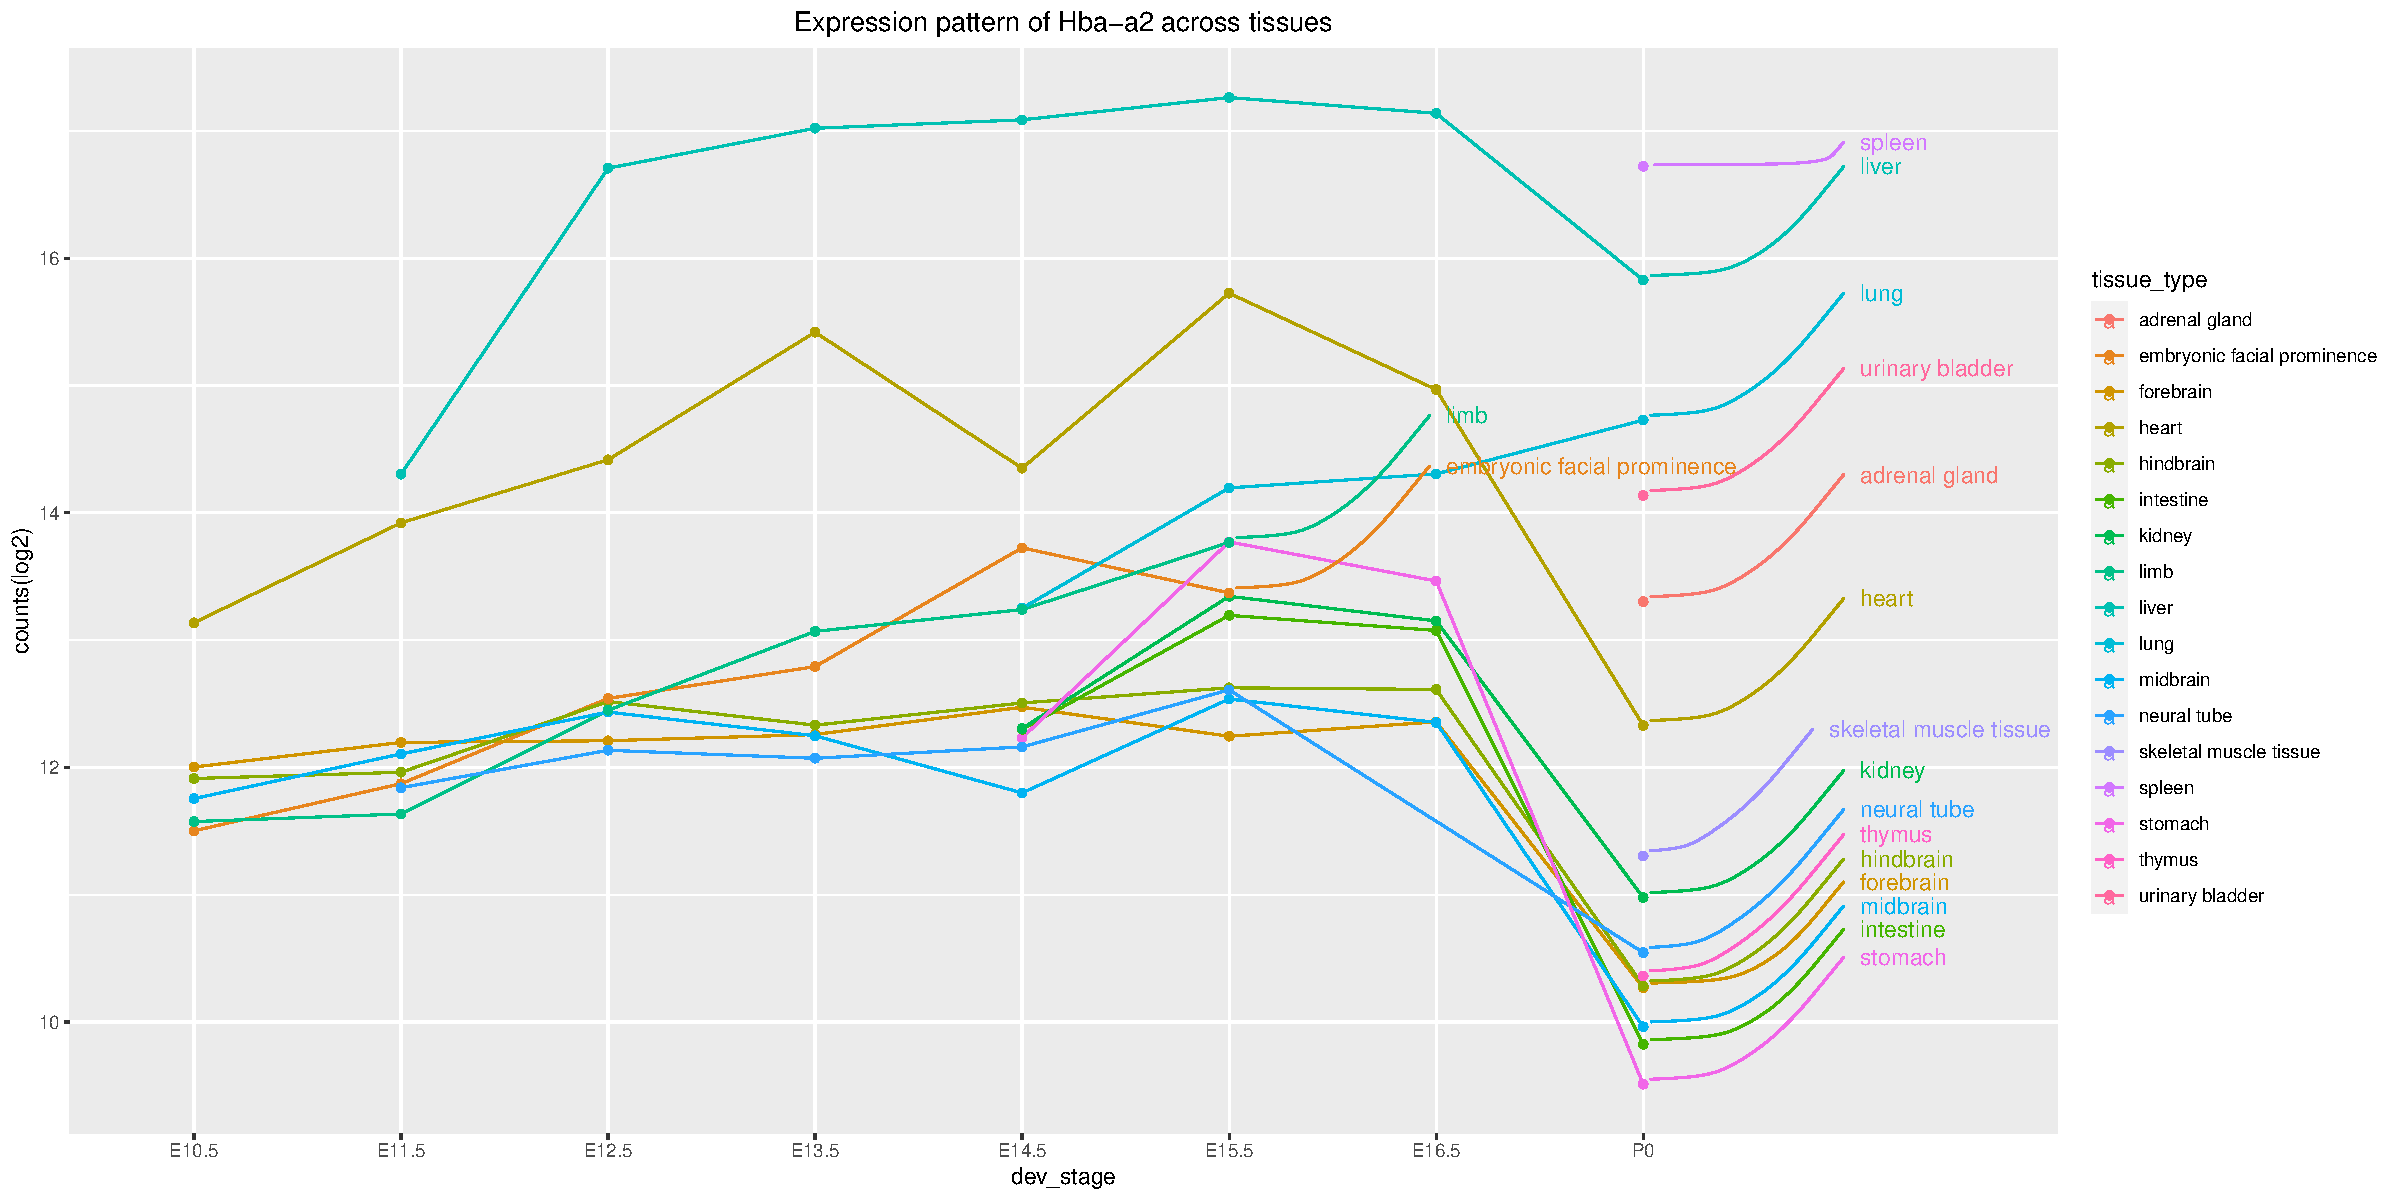
\includegraphics{Exploration_files/figure-latex/unnamed-chunk-6-1.pdf}
Top 5 Universally highly expressed protein across all tissues regardless
of stages (by percentage in tissues)

\begin{Shaded}
\begin{Highlighting}[]
\DocumentationTok{\#\#Collapse dev\_stages}
\NormalTok{collapsed\_matrices }\OtherTok{\textless{}{-}} \FunctionTok{matrix}\NormalTok{(}\AttributeTok{data=}\ConstantTok{NA}\NormalTok{, }\AttributeTok{nrow =} \FunctionTok{nrow}\NormalTok{(all\_counts), }\AttributeTok{ncol =} \FunctionTok{length}\NormalTok{(tissue\_types))}
\FunctionTok{rownames}\NormalTok{(collapsed\_matrices) }\OtherTok{\textless{}{-}} \FunctionTok{rownames}\NormalTok{(all\_counts)}
\NormalTok{walker }\OtherTok{\textless{}{-}} \DecValTok{1}
\ControlFlowTok{for}\NormalTok{ (tissue }\ControlFlowTok{in}\NormalTok{ tissue\_types)\{}
\NormalTok{  tissue\_subset\_ids }\OtherTok{\textless{}{-}}\NormalTok{ meta }\SpecialCharTok{\%\textgreater{}\%} \FunctionTok{filter}\NormalTok{(tissue\_type }\SpecialCharTok{==}\NormalTok{ tissue) }\SpecialCharTok{\%\textgreater{}\%} \FunctionTok{pull}\NormalTok{(id)}
\NormalTok{  all\_avgs }\OtherTok{\textless{}{-}} \FunctionTok{apply}\NormalTok{(all\_counts[,tissue\_subset\_ids],}\DecValTok{1}\NormalTok{, mean)}
\NormalTok{  percent\_counts }\OtherTok{\textless{}{-}}\NormalTok{ all\_avgs}\SpecialCharTok{/}\FunctionTok{sum}\NormalTok{(all\_avgs)}
\NormalTok{  collapsed\_matrices[,walker] }\OtherTok{\textless{}{-}}\NormalTok{ percent\_counts}
\NormalTok{  walker }\OtherTok{\textless{}{-}}\NormalTok{ walker }\SpecialCharTok{+} \DecValTok{1}
\NormalTok{\}}
\NormalTok{all\_sums }\OtherTok{\textless{}{-}} \FunctionTok{apply}\NormalTok{(collapsed\_matrices,}\DecValTok{1}\NormalTok{, sum)}
\ControlFlowTok{for}\NormalTok{ (i }\ControlFlowTok{in} \DecValTok{1}\SpecialCharTok{:}\DecValTok{10}\NormalTok{)\{}
  \FunctionTok{print}\NormalTok{(}\FunctionTok{paste0}\NormalTok{(}\StringTok{"The highests expressed protein acrossed all tissue in order "}\NormalTok{,i ,}\StringTok{": "}\NormalTok{, }\FunctionTok{names}\NormalTok{(}\FunctionTok{sort}\NormalTok{(all\_sums,}\AttributeTok{decreasing=}\ConstantTok{TRUE}\NormalTok{))[i]))}
\NormalTok{\}}
\end{Highlighting}
\end{Shaded}

\begin{verbatim}
## [1] "The highests expressed protein acrossed all tissue in order 1: Hba-a2"
## [1] "The highests expressed protein acrossed all tissue in order 2: Hbb-bs"
## [1] "The highests expressed protein acrossed all tissue in order 3: mt-Atp6"
## [1] "The highests expressed protein acrossed all tissue in order 4: Hba-a1"
## [1] "The highests expressed protein acrossed all tissue in order 5: mt-Atp8"
## [1] "The highests expressed protein acrossed all tissue in order 6: Hbb-bt"
## [1] "The highests expressed protein acrossed all tissue in order 7: Actb"
## [1] "The highests expressed protein acrossed all tissue in order 8: Ftl1"
## [1] "The highests expressed protein acrossed all tissue in order 9: Ppia"
## [1] "The highests expressed protein acrossed all tissue in order 10: Acta1"
\end{verbatim}

Top 5 Universally highly expressed protein across all tissues regardless
of stages (by ranking)

\begin{Shaded}
\begin{Highlighting}[]
\DocumentationTok{\#\#Collapse dev\_stages}
\NormalTok{collapsed\_matrices }\OtherTok{\textless{}{-}} \FunctionTok{matrix}\NormalTok{(}\AttributeTok{data=}\ConstantTok{NA}\NormalTok{, }\AttributeTok{nrow =} \FunctionTok{nrow}\NormalTok{(all\_counts), }\AttributeTok{ncol =} \FunctionTok{length}\NormalTok{(tissue\_types))}
\FunctionTok{rownames}\NormalTok{(collapsed\_matrices) }\OtherTok{\textless{}{-}} \FunctionTok{rownames}\NormalTok{(all\_counts)}
\NormalTok{walker }\OtherTok{\textless{}{-}} \DecValTok{1}
\ControlFlowTok{for}\NormalTok{ (tissue }\ControlFlowTok{in}\NormalTok{ tissue\_types)\{}
\NormalTok{  tissue\_subset\_ids }\OtherTok{\textless{}{-}}\NormalTok{ meta }\SpecialCharTok{\%\textgreater{}\%} \FunctionTok{filter}\NormalTok{(tissue\_type }\SpecialCharTok{==}\NormalTok{ tissue) }\SpecialCharTok{\%\textgreater{}\%} \FunctionTok{pull}\NormalTok{(id)}
\NormalTok{  all\_avgs }\OtherTok{\textless{}{-}} \FunctionTok{apply}\NormalTok{(all\_counts[,tissue\_subset\_ids],}\DecValTok{1}\NormalTok{, mean)}
\NormalTok{  all\_ranking }\OtherTok{\textless{}{-}} \FunctionTok{rank}\NormalTok{(all\_avgs)}
\NormalTok{  collapsed\_matrices[,walker] }\OtherTok{\textless{}{-}}\NormalTok{ all\_ranking}
\NormalTok{  walker }\OtherTok{\textless{}{-}}\NormalTok{ walker }\SpecialCharTok{+} \DecValTok{1}
\NormalTok{\}}
\NormalTok{all\_sums }\OtherTok{\textless{}{-}} \FunctionTok{apply}\NormalTok{(collapsed\_matrices,}\DecValTok{1}\NormalTok{, sum)}
\ControlFlowTok{for}\NormalTok{ (i }\ControlFlowTok{in} \DecValTok{1}\SpecialCharTok{:}\DecValTok{10}\NormalTok{)\{}
  \FunctionTok{print}\NormalTok{(}\FunctionTok{paste0}\NormalTok{(}\StringTok{"The highests expressed protein acrossed all tissue in order "}\NormalTok{,i ,}\StringTok{": "}\NormalTok{, }\FunctionTok{names}\NormalTok{(}\FunctionTok{sort}\NormalTok{(all\_sums, }\AttributeTok{decreasing =} \ConstantTok{TRUE}\NormalTok{))[i]))}
\NormalTok{\}}
\end{Highlighting}
\end{Shaded}

\begin{verbatim}
## [1] "The highests expressed protein acrossed all tissue in order 1: mt-Atp6"
## [1] "The highests expressed protein acrossed all tissue in order 2: mt-Atp8"
## [1] "The highests expressed protein acrossed all tissue in order 3: Hba-a2"
## [1] "The highests expressed protein acrossed all tissue in order 4: Actb"
## [1] "The highests expressed protein acrossed all tissue in order 5: Ppia"
## [1] "The highests expressed protein acrossed all tissue in order 6: Ftl1"
## [1] "The highests expressed protein acrossed all tissue in order 7: mt-Nd1"
## [1] "The highests expressed protein acrossed all tissue in order 8: Eef1a1"
## [1] "The highests expressed protein acrossed all tissue in order 9: mt-Cytb"
## [1] "The highests expressed protein acrossed all tissue in order 10: mt-Co1"
\end{verbatim}

expression distribution acrossed different tissues (box plot)

\begin{Shaded}
\begin{Highlighting}[]
\FunctionTok{library}\NormalTok{(cowplot)}
\NormalTok{all\_counts\_melted }\OtherTok{\textless{}{-}} \FunctionTok{data.frame}\NormalTok{(all\_counts) }\SpecialCharTok{\%\textgreater{}\%} \FunctionTok{gather}\NormalTok{(}\StringTok{"id"}\NormalTok{, }\StringTok{"count"}\NormalTok{)}
\NormalTok{all\_counts\_melted }\OtherTok{\textless{}{-}}\NormalTok{ all\_counts\_melted }\SpecialCharTok{\%\textgreater{}\%} \FunctionTok{inner\_join}\NormalTok{((meta }\SpecialCharTok{\%\textgreater{}\%} \FunctionTok{select}\NormalTok{(id, tissue\_type, dev\_stage)), }\AttributeTok{by=}\StringTok{"id"}\NormalTok{)}
  \FunctionTok{ggplot}\NormalTok{(}\AttributeTok{data=}\NormalTok{all\_counts\_melted, }\FunctionTok{aes}\NormalTok{(}\AttributeTok{x=}\NormalTok{dev\_stage, }\AttributeTok{y=}\FunctionTok{log2}\NormalTok{(count}\SpecialCharTok{+}\DecValTok{1}\NormalTok{))) }\SpecialCharTok{+} \FunctionTok{geom\_boxplot}\NormalTok{() }\SpecialCharTok{+}  \FunctionTok{facet\_wrap}\NormalTok{(}\SpecialCharTok{\textasciitilde{}}\NormalTok{ tissue\_type, }\AttributeTok{ncol=}\DecValTok{3}\NormalTok{) }\SpecialCharTok{+} \FunctionTok{theme\_cowplot}\NormalTok{(}\DecValTok{12}\NormalTok{) }\SpecialCharTok{+} \FunctionTok{geom\_hline}\NormalTok{(}\AttributeTok{yintercept=}\FunctionTok{median}\NormalTok{(}\FunctionTok{log2}\NormalTok{(all\_counts}\SpecialCharTok{+}\DecValTok{1}\NormalTok{)), }\AttributeTok{colour=}\StringTok{"red"}\NormalTok{)}
\end{Highlighting}
\end{Shaded}

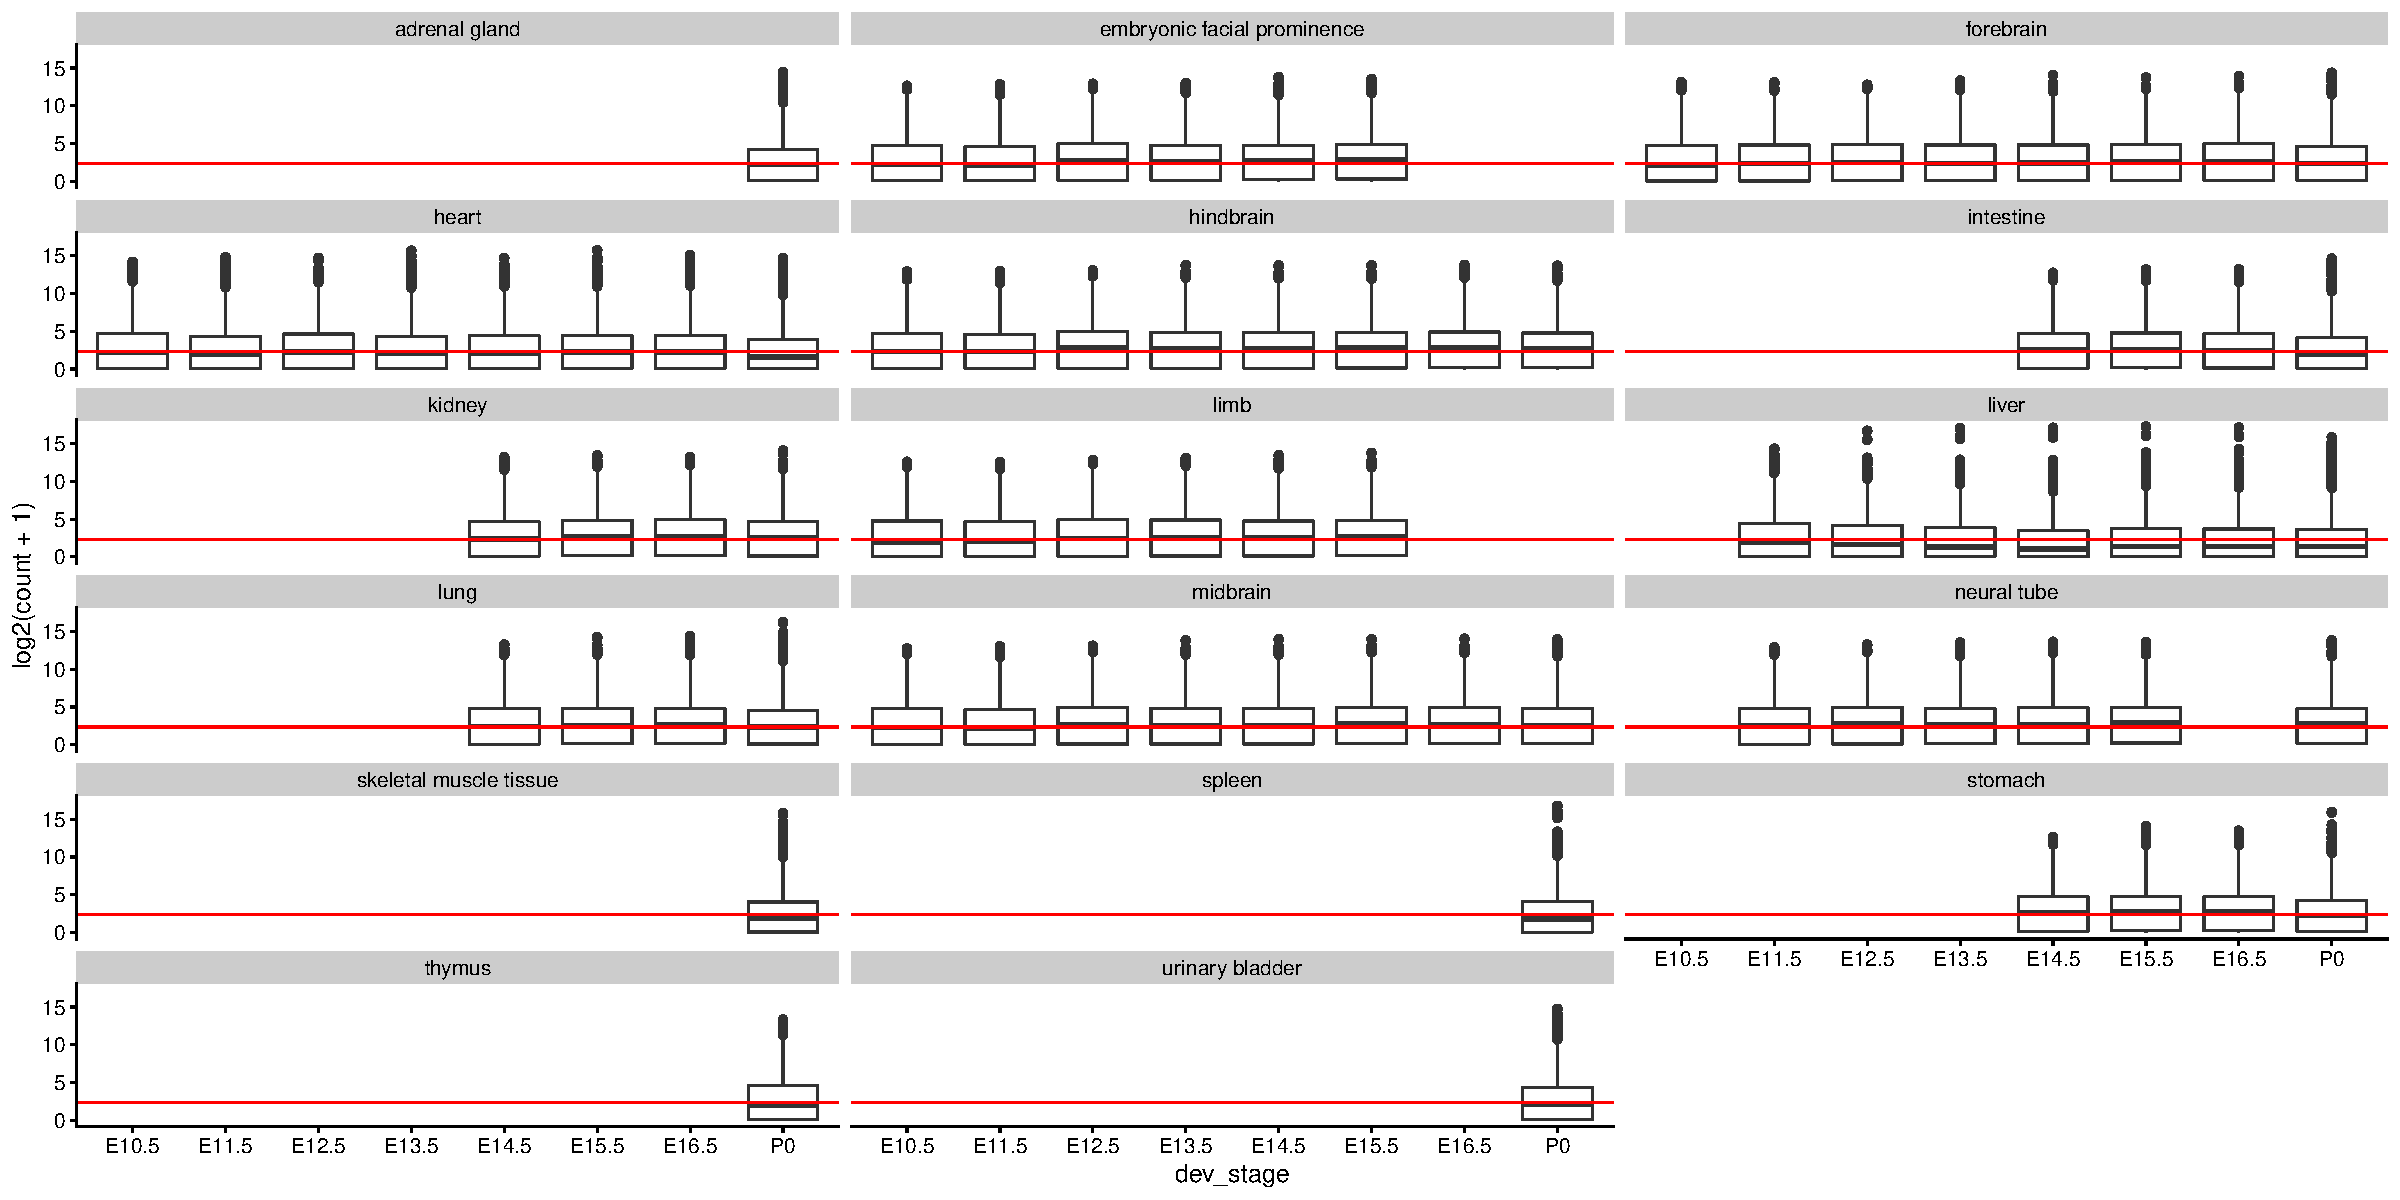
\includegraphics{Exploration_files/figure-latex/unnamed-chunk-9-1.pdf}
expression distribution acrossed different tissues (histogram)

\begin{Shaded}
\begin{Highlighting}[]
\NormalTok{all\_counts\_melted }\OtherTok{\textless{}{-}} \FunctionTok{data.frame}\NormalTok{(all\_counts) }\SpecialCharTok{\%\textgreater{}\%} \FunctionTok{gather}\NormalTok{(}\StringTok{"id"}\NormalTok{, }\StringTok{"count"}\NormalTok{)}
\NormalTok{all\_counts\_melted }\OtherTok{\textless{}{-}}\NormalTok{ all\_counts\_melted }\SpecialCharTok{\%\textgreater{}\%} \FunctionTok{inner\_join}\NormalTok{((meta }\SpecialCharTok{\%\textgreater{}\%} \FunctionTok{select}\NormalTok{(id, tissue\_type, dev\_stage)), }\AttributeTok{by=}\StringTok{"id"}\NormalTok{)}
  \FunctionTok{suppressWarnings}\NormalTok{(}\FunctionTok{ggplot}\NormalTok{(}\AttributeTok{data=}\NormalTok{all\_counts\_melted, }\FunctionTok{aes}\NormalTok{(}\AttributeTok{x=}\FunctionTok{log2}\NormalTok{(count}\SpecialCharTok{+}\DecValTok{1}\NormalTok{), }\AttributeTok{fill=}\NormalTok{dev\_stage)) }\SpecialCharTok{+} \FunctionTok{geom\_histogram}\NormalTok{(}\AttributeTok{binwidth =} \FloatTok{0.5}\NormalTok{) }\SpecialCharTok{+}  \FunctionTok{facet\_wrap}\NormalTok{(}\SpecialCharTok{\textasciitilde{}}\NormalTok{ tissue\_type, }\AttributeTok{ncol=}\DecValTok{3}\NormalTok{) }\SpecialCharTok{+} \FunctionTok{theme\_cowplot}\NormalTok{(}\DecValTok{12}\NormalTok{))}
\end{Highlighting}
\end{Shaded}

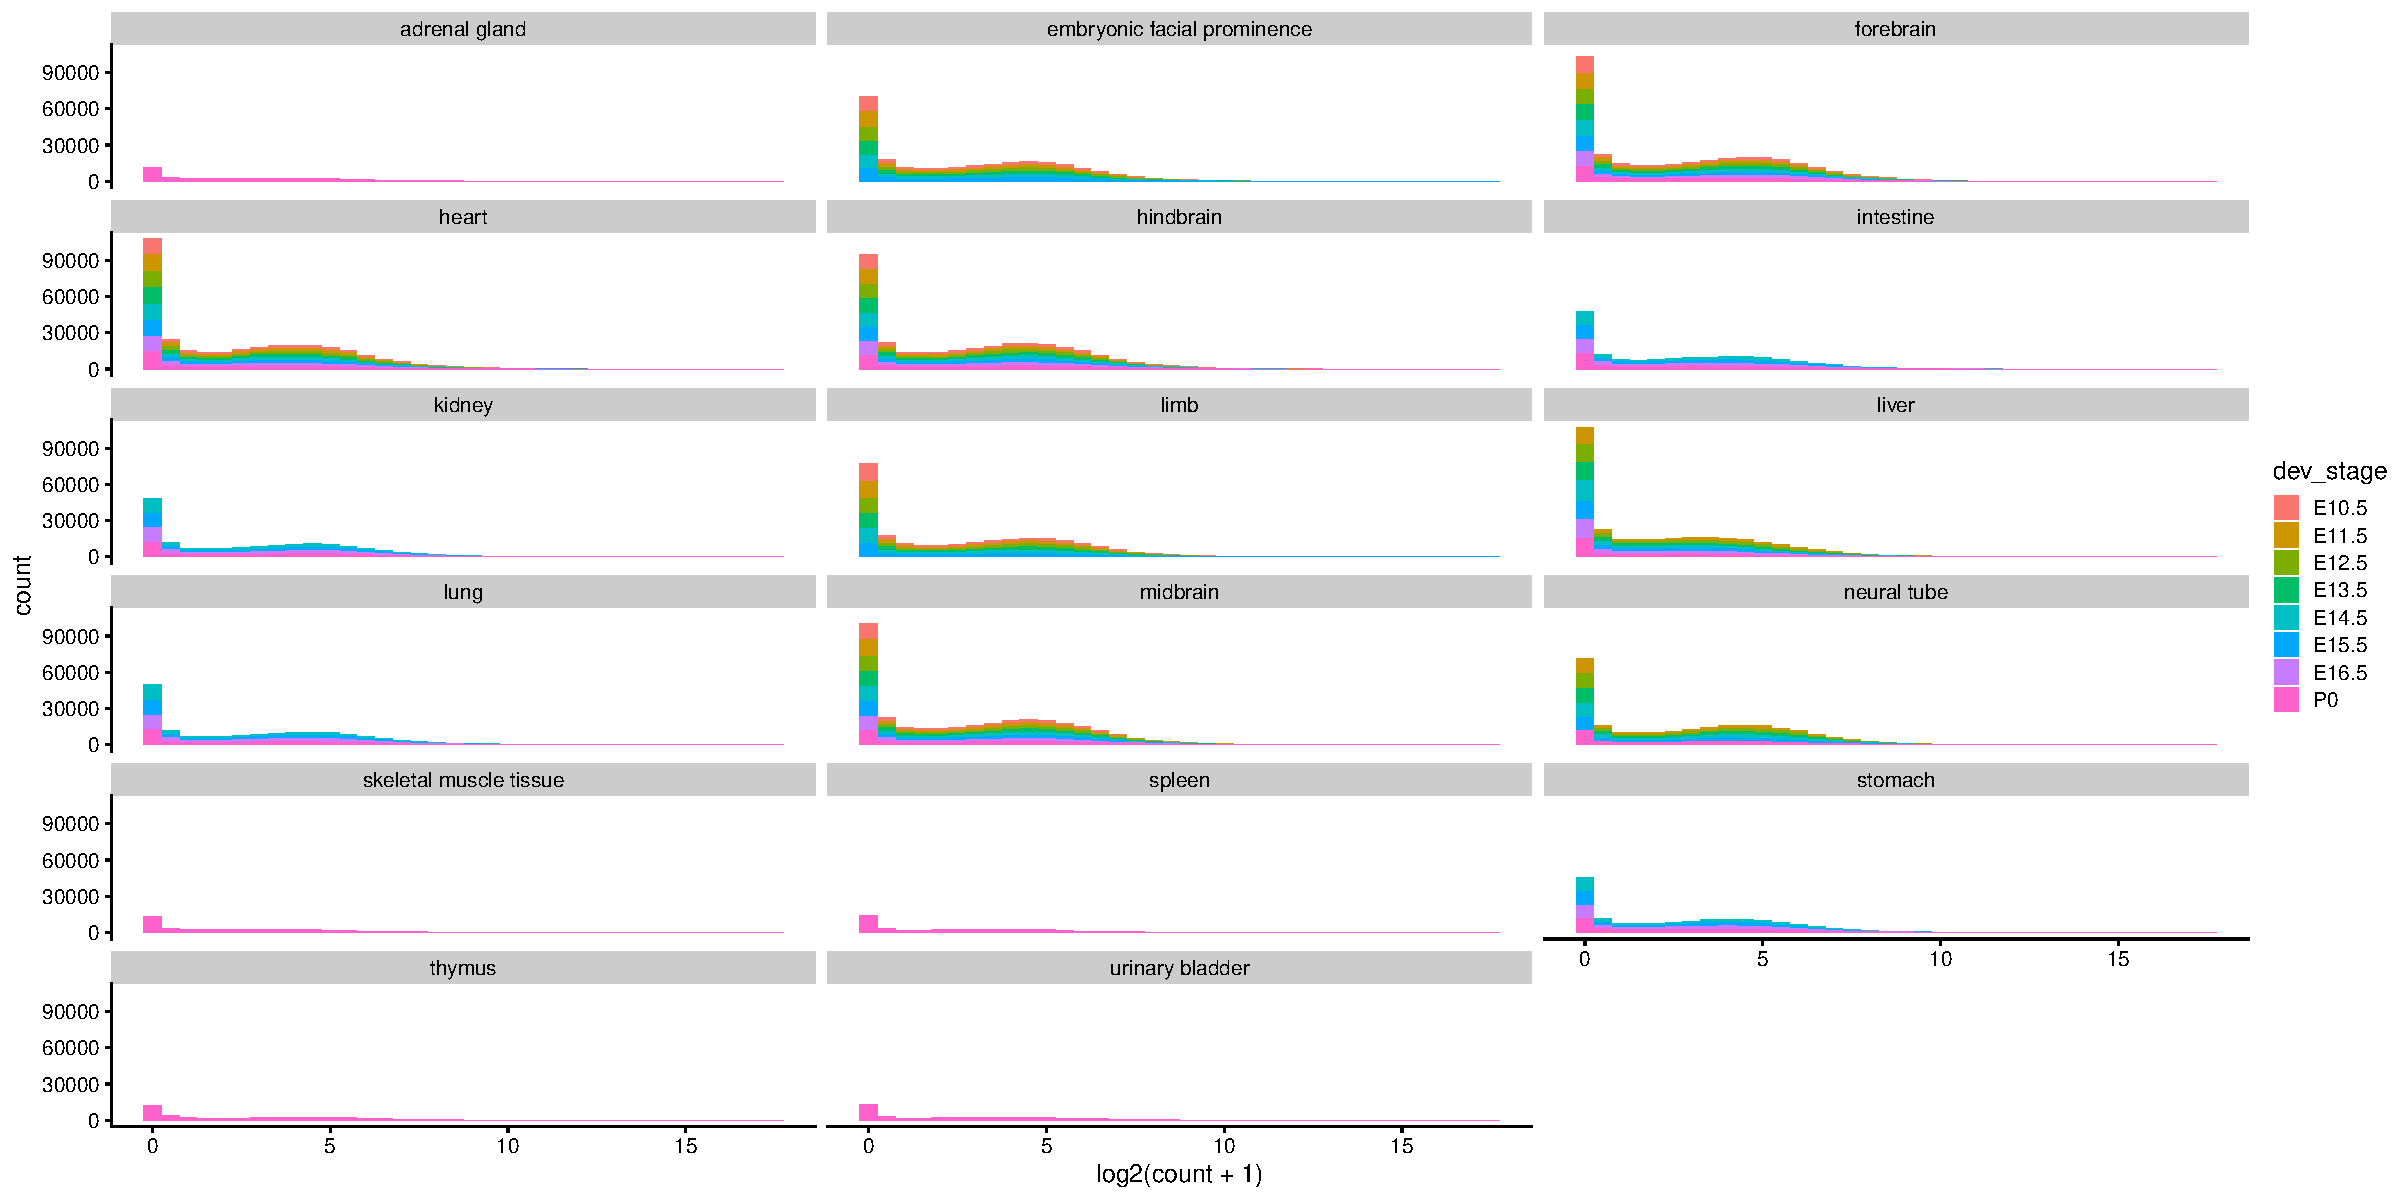
\includegraphics{Exploration_files/figure-latex/unnamed-chunk-10-1.pdf}

expression distribution acrossed different tissues (histogram log
transformed)

\begin{Shaded}
\begin{Highlighting}[]
\NormalTok{all\_counts\_melted }\OtherTok{\textless{}{-}} \FunctionTok{data.frame}\NormalTok{(all\_counts) }\SpecialCharTok{\%\textgreater{}\%} \FunctionTok{gather}\NormalTok{(}\StringTok{"id"}\NormalTok{, }\StringTok{"count"}\NormalTok{)}
\NormalTok{all\_counts\_melted }\OtherTok{\textless{}{-}}\NormalTok{ all\_counts\_melted }\SpecialCharTok{\%\textgreater{}\%} \FunctionTok{inner\_join}\NormalTok{((meta }\SpecialCharTok{\%\textgreater{}\%} \FunctionTok{select}\NormalTok{(id, tissue\_type, dev\_stage)), }\AttributeTok{by=}\StringTok{"id"}\NormalTok{)}
  \FunctionTok{suppressWarnings}\NormalTok{(}\FunctionTok{ggplot}\NormalTok{(}\AttributeTok{data=}\NormalTok{all\_counts\_melted, }\FunctionTok{aes}\NormalTok{(}\AttributeTok{x=}\FunctionTok{log2}\NormalTok{(count}\SpecialCharTok{+}\DecValTok{1}\NormalTok{), }\AttributeTok{y=}\NormalTok{..density.. ,}\AttributeTok{fill=}\NormalTok{dev\_stage)) }\SpecialCharTok{+} \FunctionTok{geom\_histogram}\NormalTok{(}\AttributeTok{binwidth =} \FloatTok{0.5}\NormalTok{) }\SpecialCharTok{+}  \FunctionTok{facet\_wrap}\NormalTok{(}\SpecialCharTok{\textasciitilde{}}\NormalTok{ tissue\_type, }\AttributeTok{ncol=}\DecValTok{3}\NormalTok{) }\SpecialCharTok{+} \FunctionTok{theme\_cowplot}\NormalTok{(}\DecValTok{12}\NormalTok{))}
\end{Highlighting}
\end{Shaded}

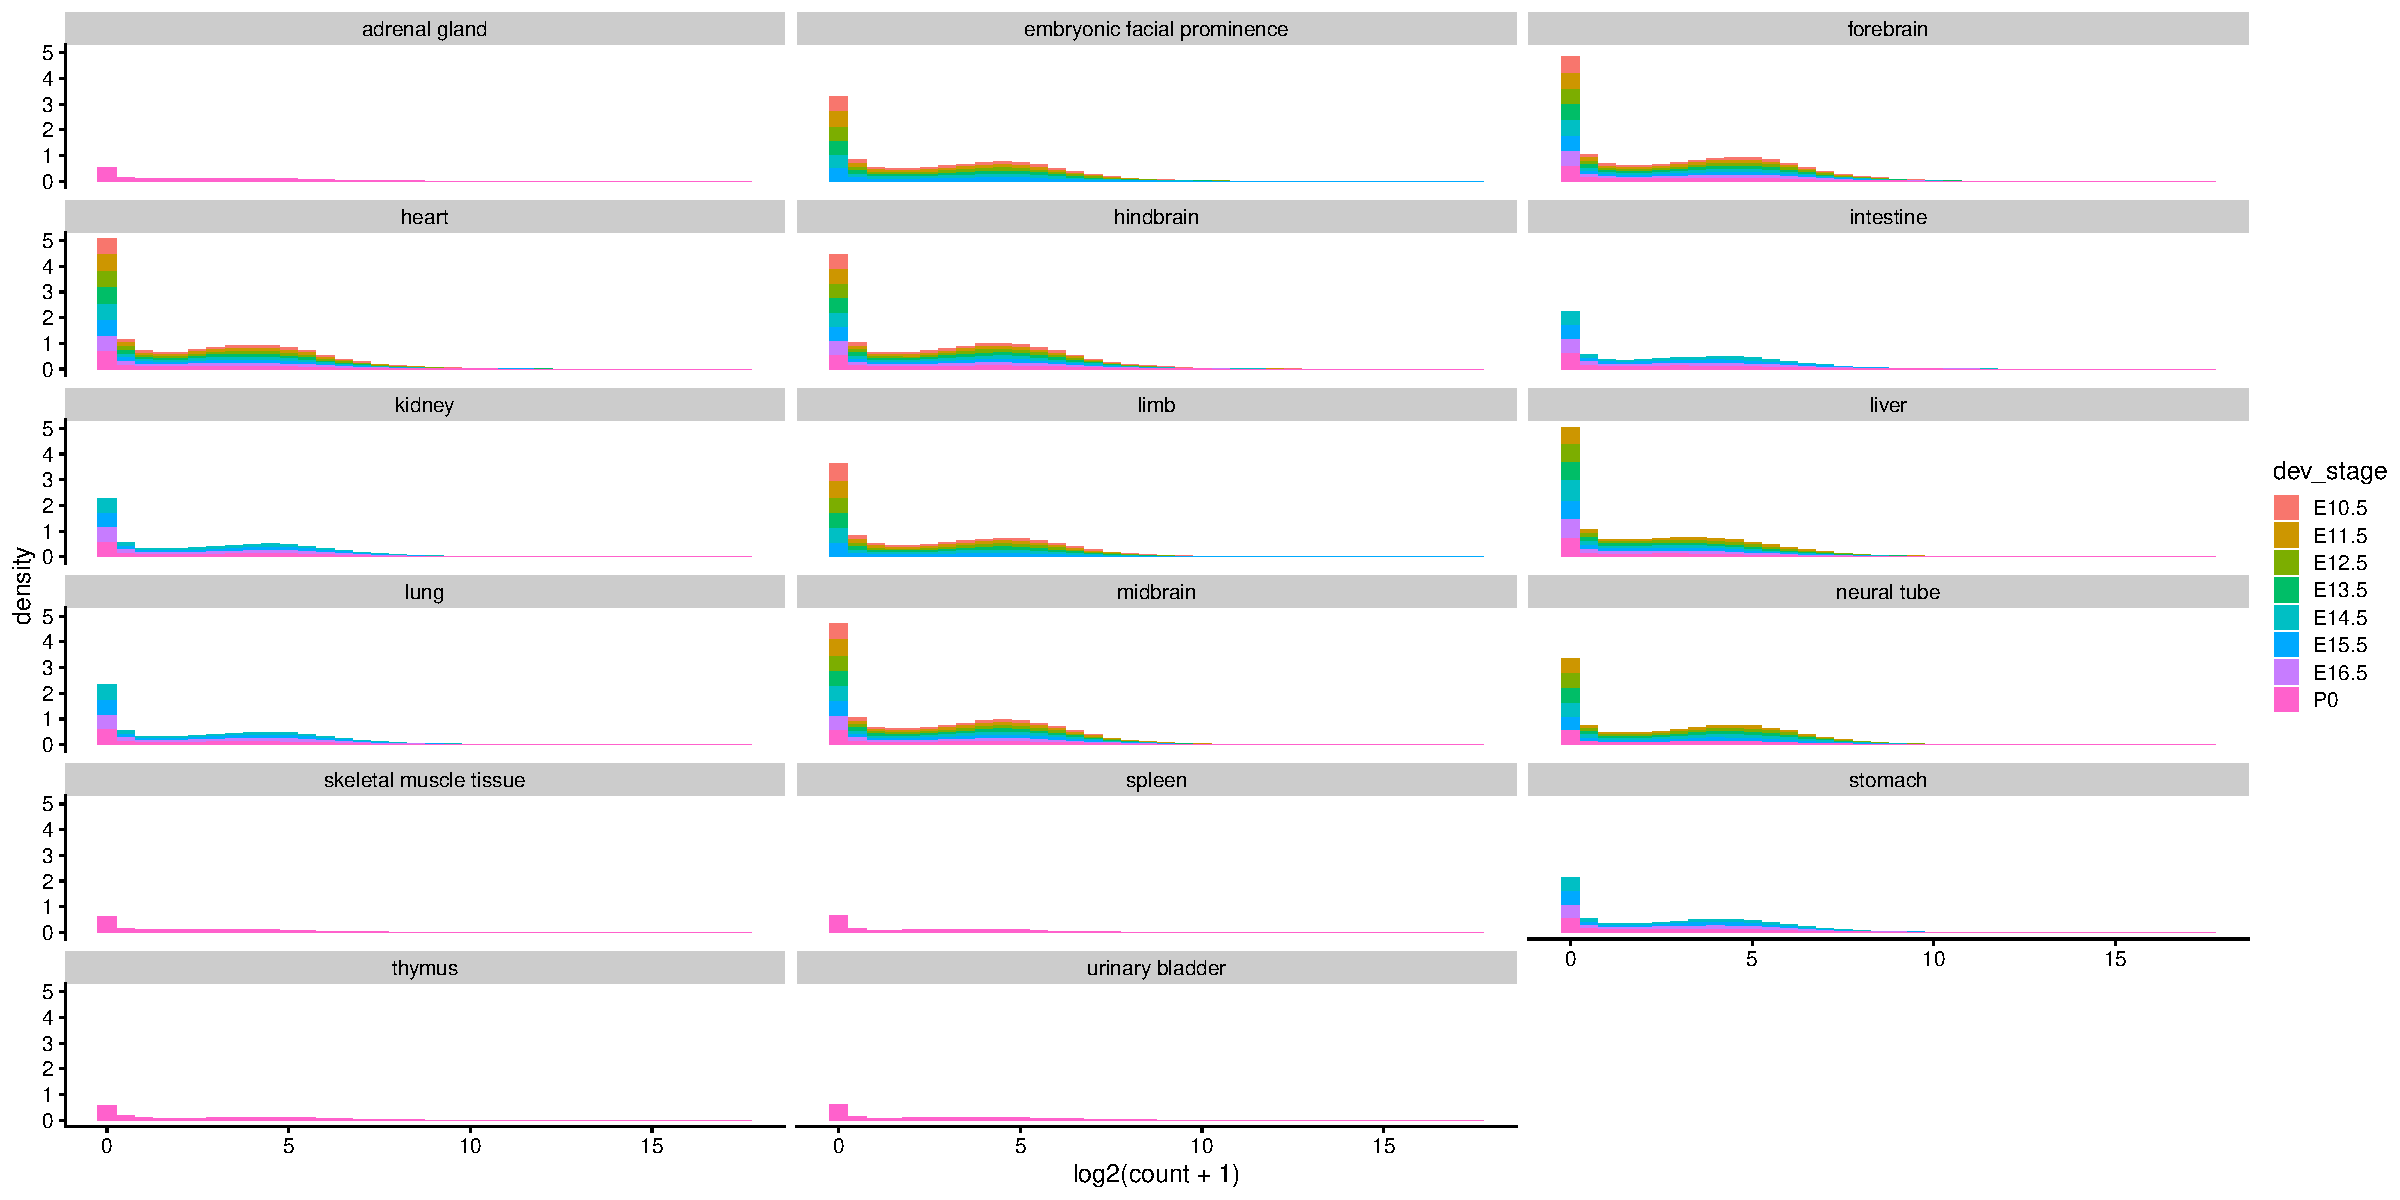
\includegraphics{Exploration_files/figure-latex/unnamed-chunk-11-1.pdf}
expression distribution acrossed different tissues (box plot collapsed
dev\_stages)

\begin{Shaded}
\begin{Highlighting}[]
\NormalTok{all\_counts\_melted }\OtherTok{\textless{}{-}} \FunctionTok{data.frame}\NormalTok{(all\_counts) }\SpecialCharTok{\%\textgreater{}\%} \FunctionTok{gather}\NormalTok{(}\StringTok{"id"}\NormalTok{, }\StringTok{"count"}\NormalTok{)}
\NormalTok{all\_counts\_melted }\OtherTok{\textless{}{-}}\NormalTok{ all\_counts\_melted }\SpecialCharTok{\%\textgreater{}\%} \FunctionTok{inner\_join}\NormalTok{((meta }\SpecialCharTok{\%\textgreater{}\%} \FunctionTok{select}\NormalTok{(id, tissue\_type, dev\_stage)), }\AttributeTok{by=}\StringTok{"id"}\NormalTok{)}
  \FunctionTok{ggplot}\NormalTok{(}\AttributeTok{data=}\NormalTok{all\_counts\_melted, }\FunctionTok{aes}\NormalTok{(}\AttributeTok{y=}\FunctionTok{log2}\NormalTok{(count}\SpecialCharTok{+}\DecValTok{1}\NormalTok{))) }\SpecialCharTok{+} \FunctionTok{geom\_boxplot}\NormalTok{() }\SpecialCharTok{+}  \FunctionTok{facet\_grid}\NormalTok{(. }\SpecialCharTok{\textasciitilde{}}\NormalTok{ tissue\_type) }\SpecialCharTok{+} \FunctionTok{theme\_cowplot}\NormalTok{(}\DecValTok{12}\NormalTok{) }\SpecialCharTok{+} \FunctionTok{theme}\NormalTok{(}
        \AttributeTok{axis.text.x=}\FunctionTok{element\_blank}\NormalTok{(),}
        \AttributeTok{axis.ticks.x=}\FunctionTok{element\_blank}\NormalTok{()) }\SpecialCharTok{+} \FunctionTok{xlab}\NormalTok{(}\StringTok{"tissue\_types"}\NormalTok{) }\SpecialCharTok{+} \FunctionTok{geom\_hline}\NormalTok{(}\AttributeTok{yintercept=}\FunctionTok{median}\NormalTok{(}\FunctionTok{log2}\NormalTok{(all\_counts}\SpecialCharTok{+}\DecValTok{1}\NormalTok{)), }\AttributeTok{colour=}\StringTok{"red"}\NormalTok{)}
\end{Highlighting}
\end{Shaded}

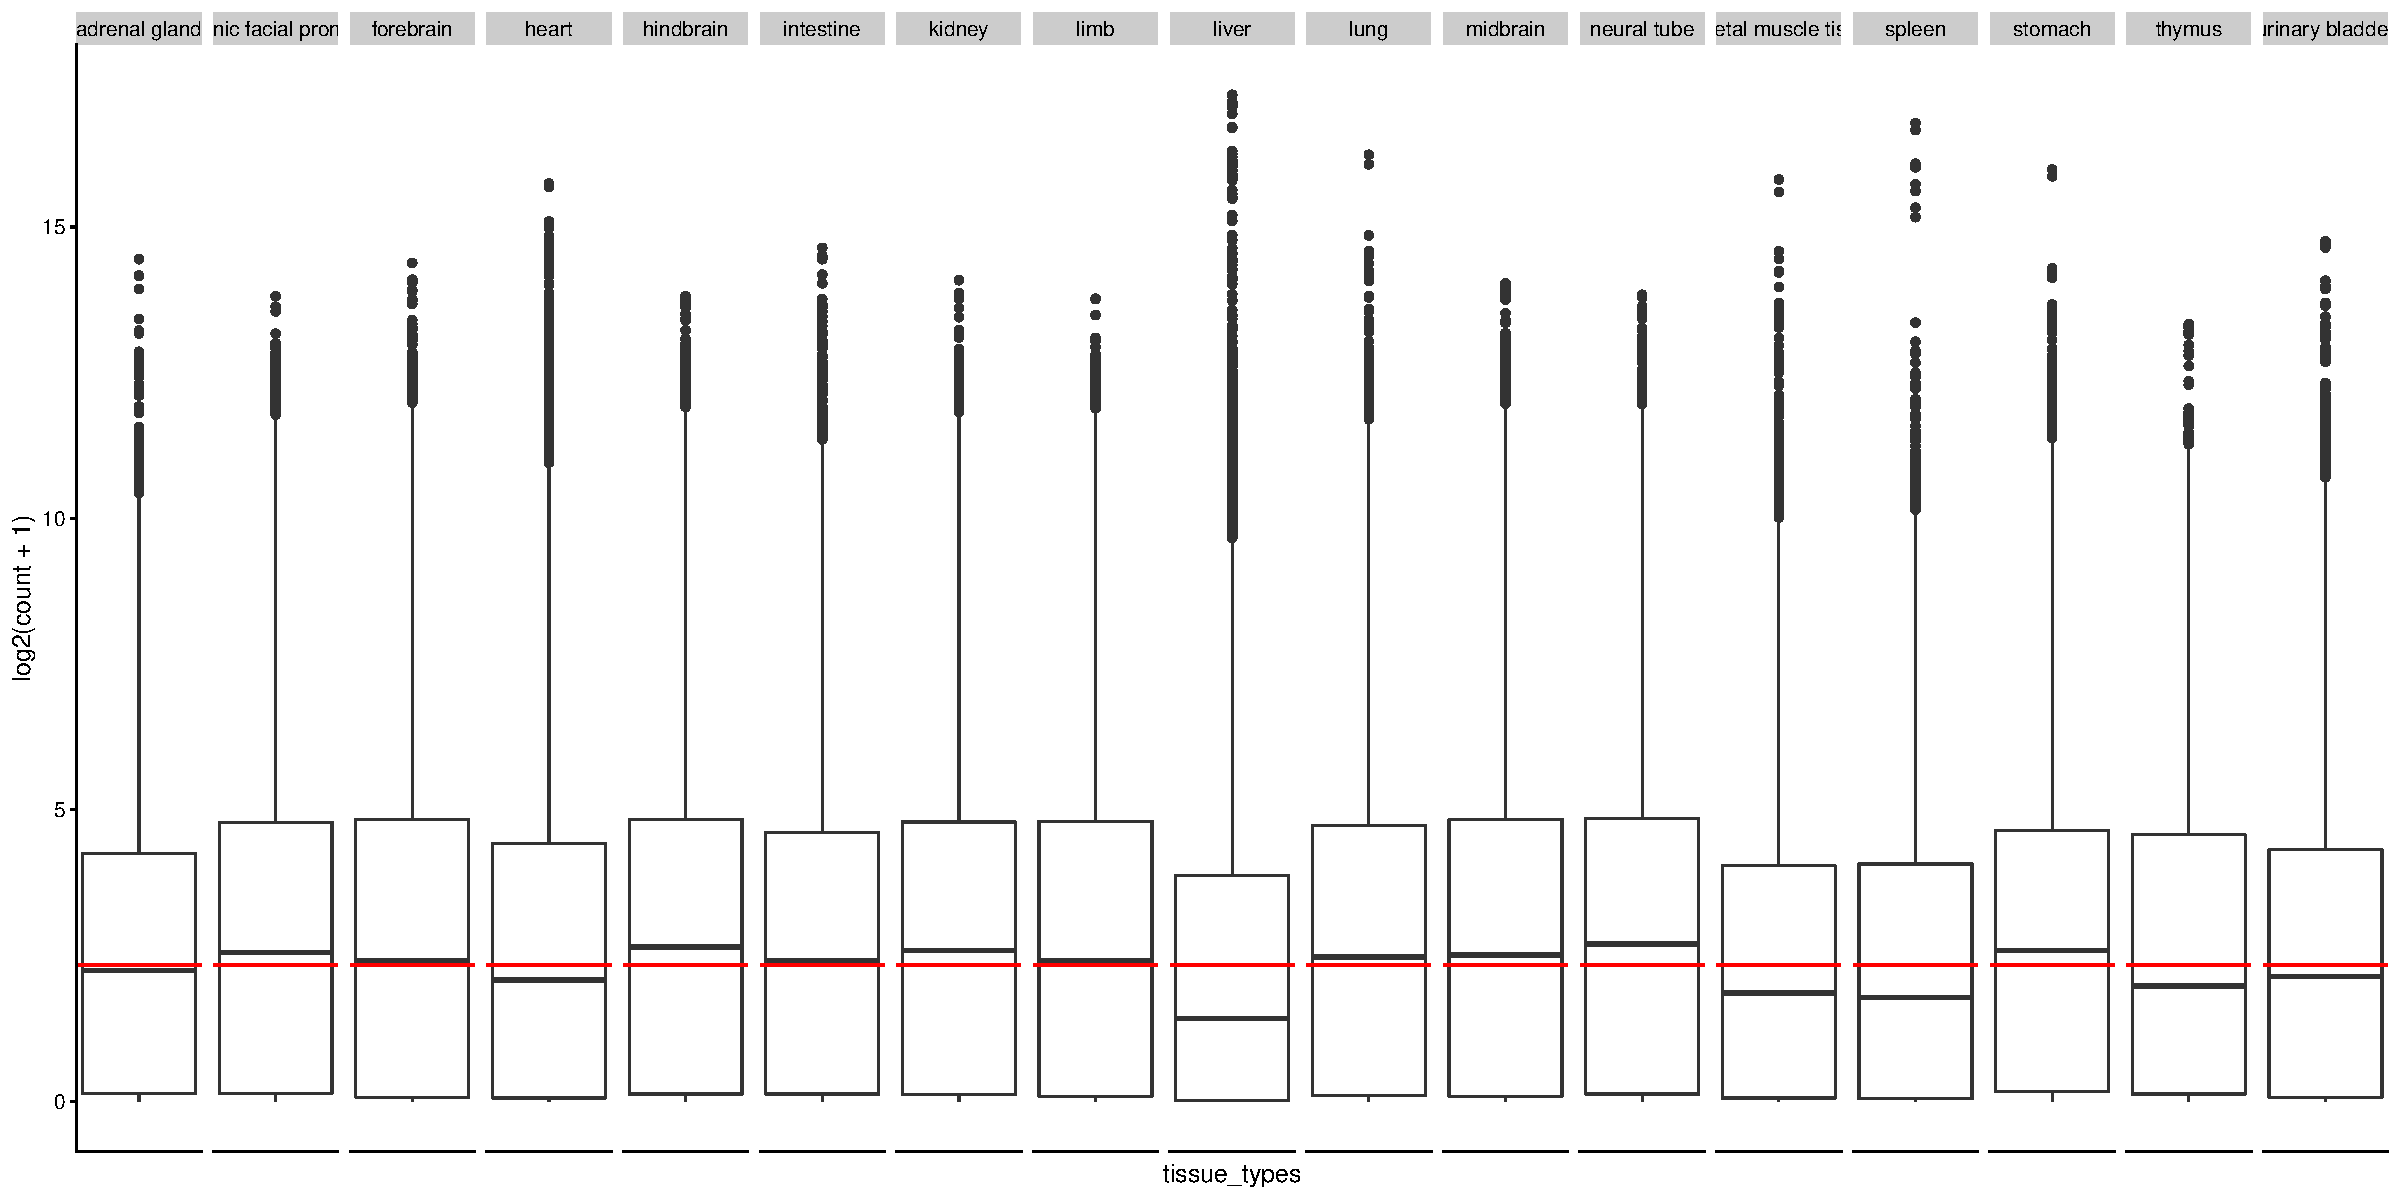
\includegraphics{Exploration_files/figure-latex/unnamed-chunk-12-1.pdf}
expression distribution acrossed different tissues (histogram collapsed
by dev\_stage)

\begin{Shaded}
\begin{Highlighting}[]
\NormalTok{all\_counts\_melted }\OtherTok{\textless{}{-}} \FunctionTok{data.frame}\NormalTok{(all\_counts) }\SpecialCharTok{\%\textgreater{}\%} \FunctionTok{gather}\NormalTok{(}\StringTok{"id"}\NormalTok{, }\StringTok{"count"}\NormalTok{)}
\NormalTok{all\_counts\_melted }\OtherTok{\textless{}{-}}\NormalTok{ all\_counts\_melted }\SpecialCharTok{\%\textgreater{}\%} \FunctionTok{inner\_join}\NormalTok{((meta }\SpecialCharTok{\%\textgreater{}\%} \FunctionTok{select}\NormalTok{(id, tissue\_type, dev\_stage)), }\AttributeTok{by=}\StringTok{"id"}\NormalTok{)}
  \FunctionTok{suppressWarnings}\NormalTok{(}\FunctionTok{ggplot}\NormalTok{(}\AttributeTok{data=}\NormalTok{all\_counts\_melted, }\FunctionTok{aes}\NormalTok{(}\AttributeTok{x=}\FunctionTok{log2}\NormalTok{(count}\SpecialCharTok{+}\DecValTok{1}\NormalTok{), }\AttributeTok{fill=}\NormalTok{tissue\_type, }\AttributeTok{y=}\NormalTok{..density..)) }\SpecialCharTok{+} \FunctionTok{geom\_histogram}\NormalTok{(}\AttributeTok{binwidth =} \FloatTok{0.5}\NormalTok{) }\SpecialCharTok{+} \FunctionTok{theme\_cowplot}\NormalTok{(}\DecValTok{12}\NormalTok{))  }
\end{Highlighting}
\end{Shaded}

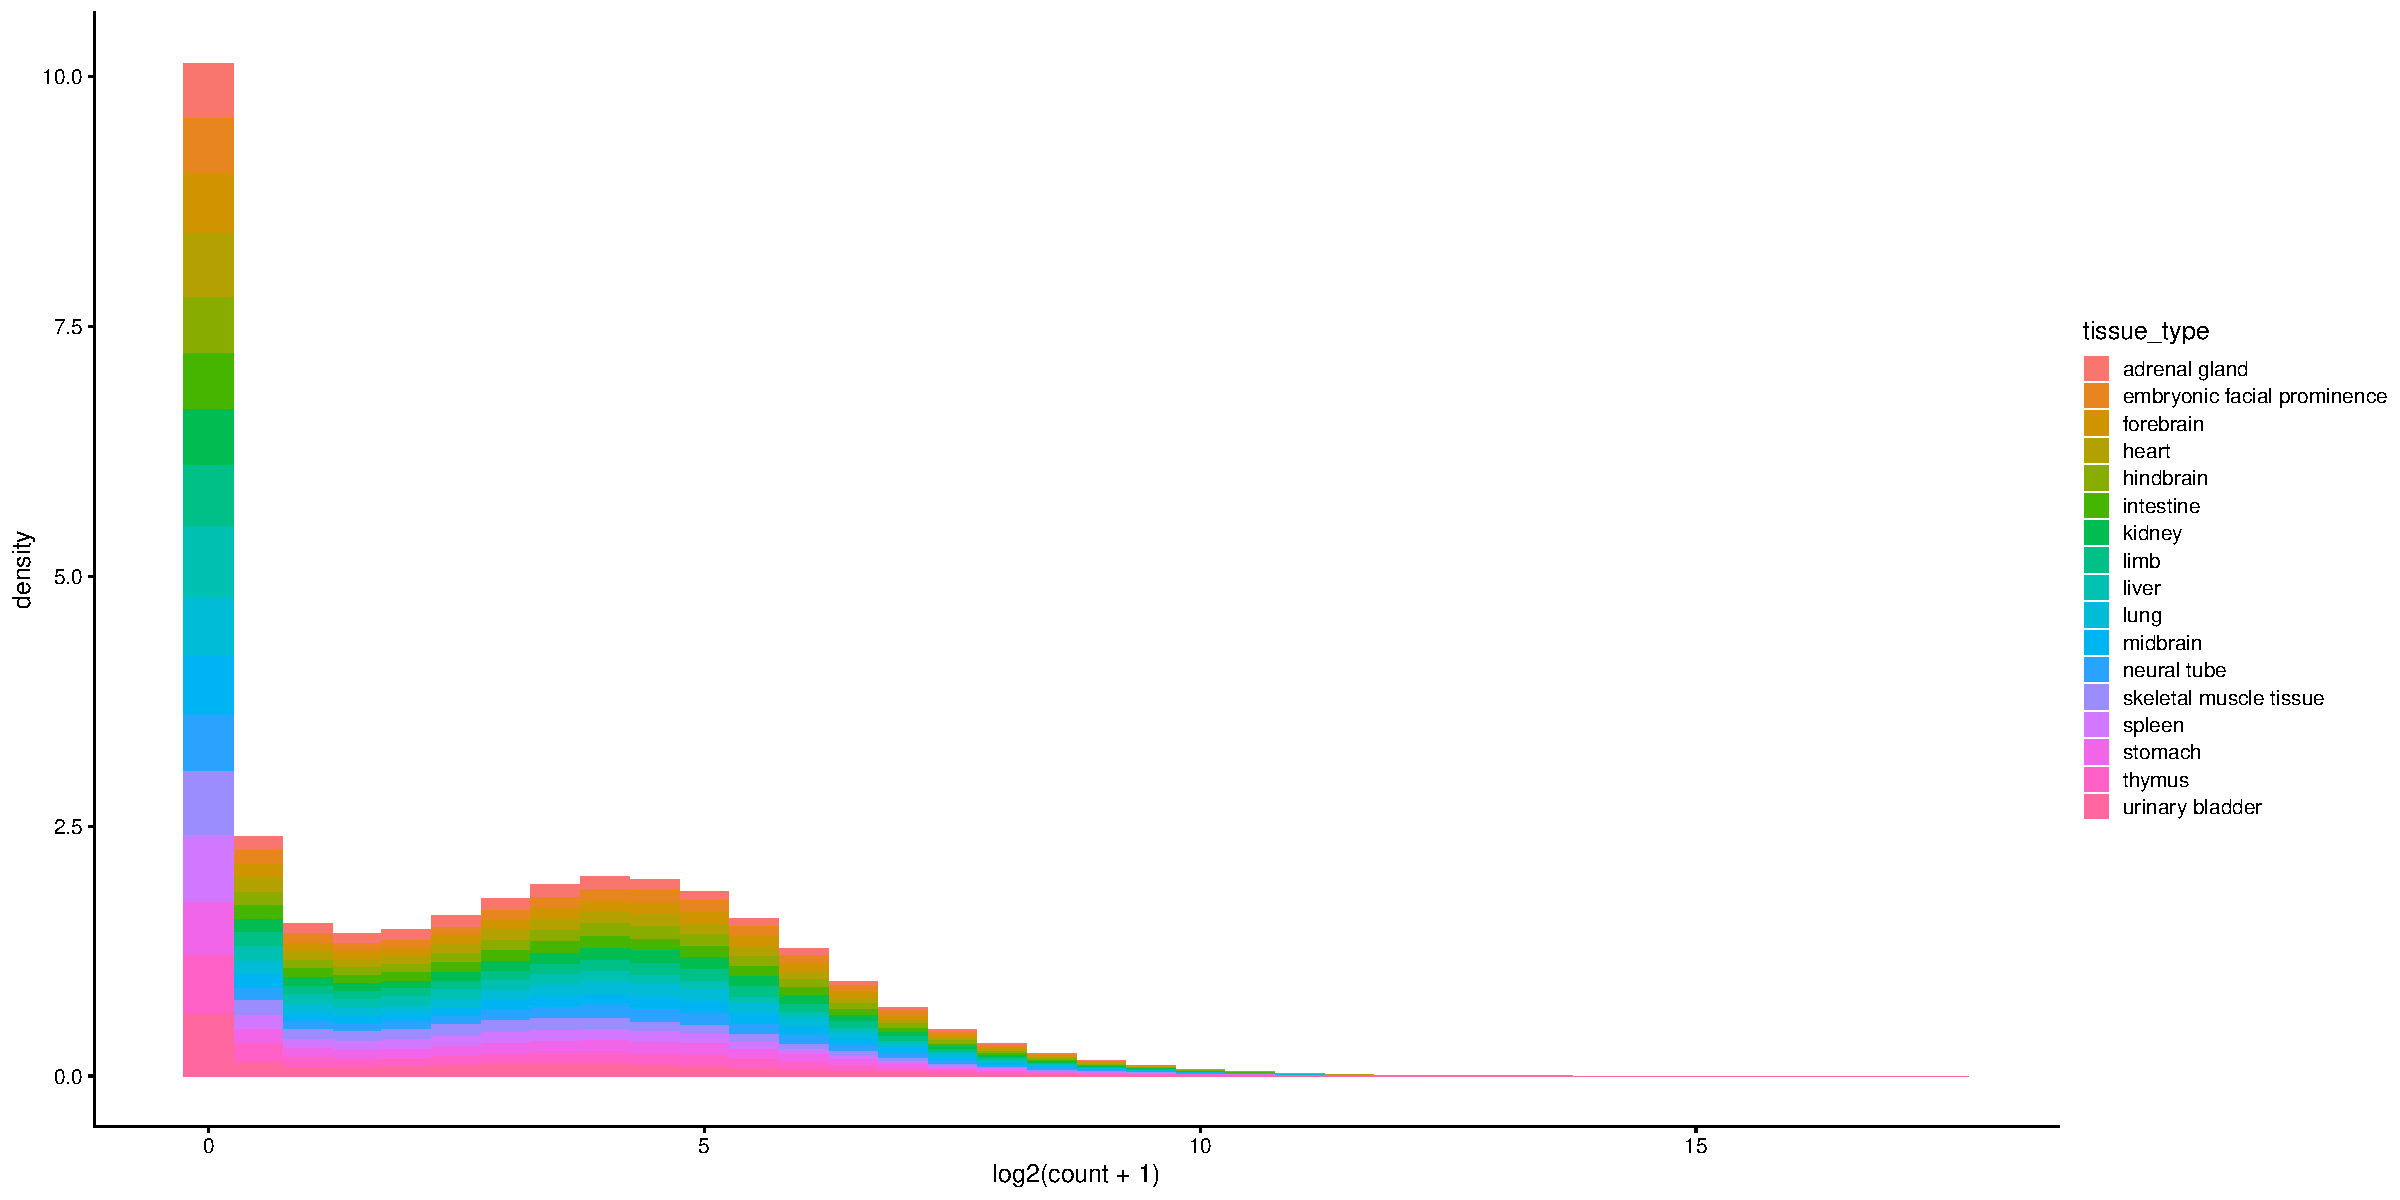
\includegraphics{Exploration_files/figure-latex/unnamed-chunk-13-1.pdf}
expression distribution acrossed different tissues (freq\_plot collapsed
by dev\_stage)

\begin{Shaded}
\begin{Highlighting}[]
\NormalTok{all\_counts\_melted }\OtherTok{\textless{}{-}} \FunctionTok{data.frame}\NormalTok{(all\_counts) }\SpecialCharTok{\%\textgreater{}\%} \FunctionTok{gather}\NormalTok{(}\StringTok{"id"}\NormalTok{, }\StringTok{"count"}\NormalTok{)}
\NormalTok{all\_counts\_melted }\OtherTok{\textless{}{-}}\NormalTok{ all\_counts\_melted }\SpecialCharTok{\%\textgreater{}\%} \FunctionTok{inner\_join}\NormalTok{((meta }\SpecialCharTok{\%\textgreater{}\%} \FunctionTok{select}\NormalTok{(id, tissue\_type, dev\_stage)), }\AttributeTok{by=}\StringTok{"id"}\NormalTok{)}
  \FunctionTok{ggplot}\NormalTok{(}\AttributeTok{data=}\NormalTok{all\_counts\_melted, }\FunctionTok{aes}\NormalTok{(}\AttributeTok{x=}\FunctionTok{log2}\NormalTok{(count}\SpecialCharTok{+}\DecValTok{1}\NormalTok{), }\AttributeTok{y=}\NormalTok{..density.., }\AttributeTok{colour=}\NormalTok{tissue\_type)) }\SpecialCharTok{+} \FunctionTok{geom\_freqpoly}\NormalTok{(}\AttributeTok{binwidth=}\FloatTok{0.5}\NormalTok{) }\SpecialCharTok{+} \FunctionTok{theme\_cowplot}\NormalTok{(}\DecValTok{12}\NormalTok{) }\SpecialCharTok{+} \FunctionTok{scale\_x\_continuous}\NormalTok{(}\AttributeTok{limits=}\FunctionTok{c}\NormalTok{(}\DecValTok{0}\NormalTok{, }\DecValTok{20}\NormalTok{))}
\end{Highlighting}
\end{Shaded}

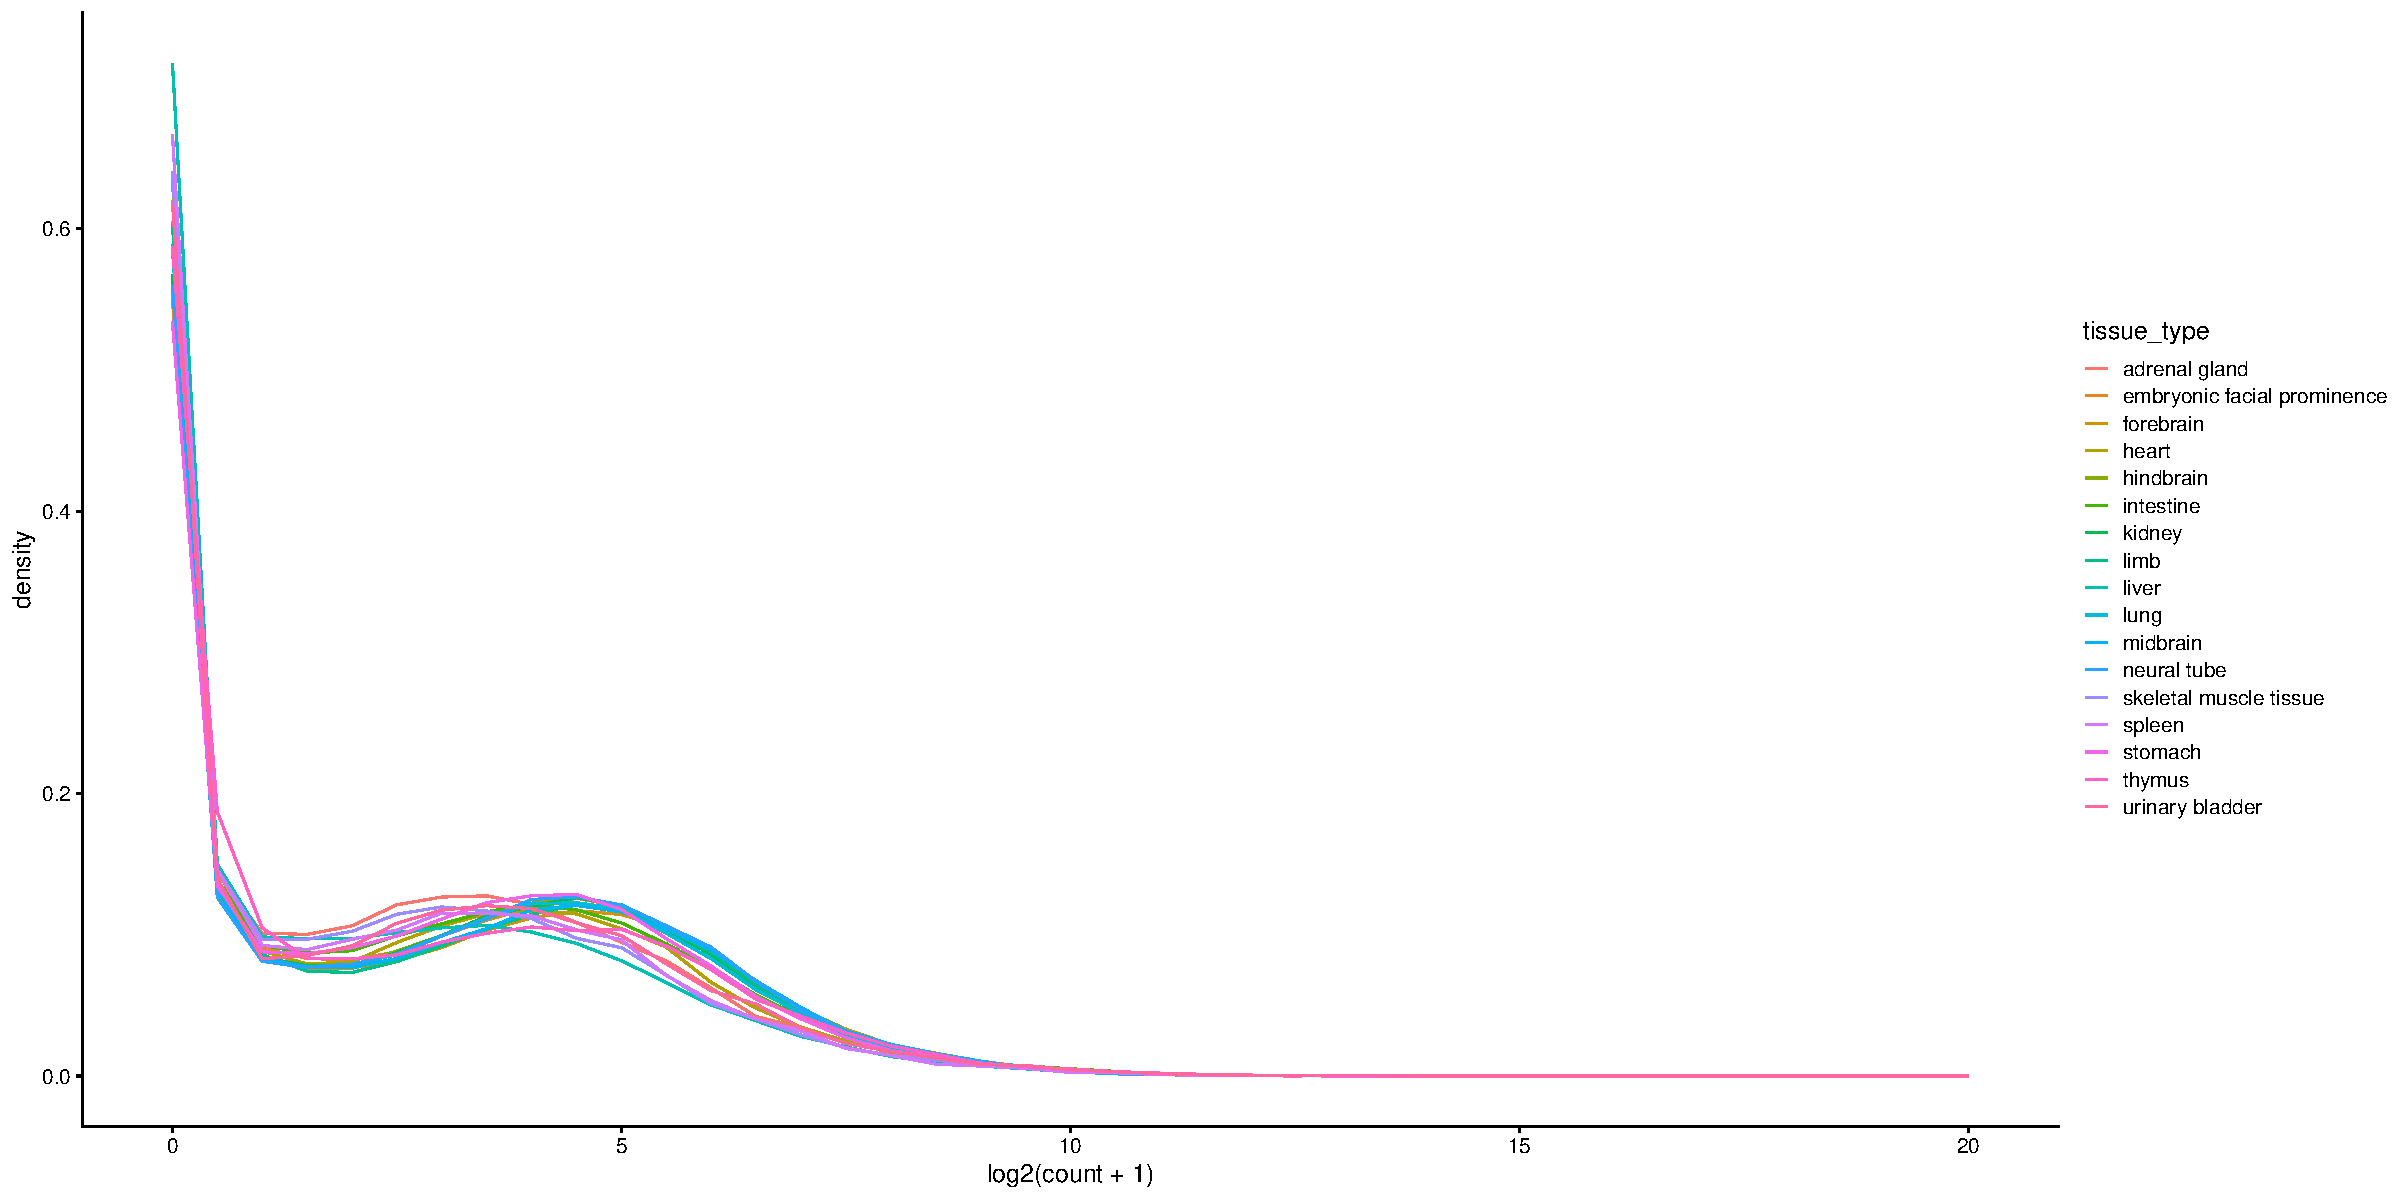
\includegraphics{Exploration_files/figure-latex/unnamed-chunk-14-1.pdf}
Mean-variance

\begin{Shaded}
\begin{Highlighting}[]
\FunctionTok{library}\NormalTok{(ggrepel)}
\NormalTok{all\_counts\_mean\_var }\OtherTok{\textless{}{-}}\NormalTok{ all\_counts}
\NormalTok{all\_counts\_mean\_var }\OtherTok{\textless{}{-}} \FunctionTok{cbind}\NormalTok{(all\_counts\_mean\_var, }\AttributeTok{mean=}\FunctionTok{apply}\NormalTok{(all\_counts,}\DecValTok{1}\NormalTok{,mean))}
\NormalTok{all\_counts\_mean\_var }\OtherTok{\textless{}{-}} \FunctionTok{cbind}\NormalTok{(all\_counts\_mean\_var, }\AttributeTok{variance=}\FunctionTok{apply}\NormalTok{(all\_counts,}\DecValTok{1}\NormalTok{,var))}
\FunctionTok{ggplot}\NormalTok{(}\AttributeTok{data=}\FunctionTok{data.frame}\NormalTok{(all\_counts\_mean\_var), }\FunctionTok{aes}\NormalTok{(}\AttributeTok{x=}\FunctionTok{log2}\NormalTok{(mean}\SpecialCharTok{+}\DecValTok{1}\NormalTok{), }\AttributeTok{y=}\FunctionTok{log2}\NormalTok{(variance}\SpecialCharTok{+}\DecValTok{1}\NormalTok{))) }\SpecialCharTok{+} \FunctionTok{geom\_point}\NormalTok{() }\SpecialCharTok{+} \FunctionTok{theme\_cowplot}\NormalTok{(}\DecValTok{12}\NormalTok{) }\SpecialCharTok{+} 
  \FunctionTok{geom\_text\_repel}\NormalTok{(}\AttributeTok{data=}\FunctionTok{data.frame}\NormalTok{(all\_counts\_mean\_var) }\SpecialCharTok{\%\textgreater{}\%} \FunctionTok{rownames\_to\_column}\NormalTok{(}\AttributeTok{var=}\StringTok{"rowname"}\NormalTok{) }\SpecialCharTok{\%\textgreater{}\%} \FunctionTok{slice\_max}\NormalTok{(variance, }\AttributeTok{n=}\DecValTok{10}\NormalTok{), }\FunctionTok{aes}\NormalTok{(}\AttributeTok{x=}\FunctionTok{log2}\NormalTok{(mean}\SpecialCharTok{+}\DecValTok{1}\NormalTok{), }\AttributeTok{y=}\FunctionTok{log2}\NormalTok{(variance), }\AttributeTok{label=}\NormalTok{rowname, }\AttributeTok{colour=}\StringTok{"red"}\NormalTok{)) }\SpecialCharTok{+}
  \FunctionTok{geom\_text\_repel}\NormalTok{(}\AttributeTok{data=}\FunctionTok{data.frame}\NormalTok{(all\_counts\_mean\_var) }\SpecialCharTok{\%\textgreater{}\%} \FunctionTok{rownames\_to\_column}\NormalTok{(}\AttributeTok{var=}\StringTok{"rowname"}\NormalTok{) }\SpecialCharTok{\%\textgreater{}\%} \FunctionTok{slice\_max}\NormalTok{(mean, }\AttributeTok{n=}\DecValTok{10}\NormalTok{), }\FunctionTok{aes}\NormalTok{(}\AttributeTok{x=}\FunctionTok{log2}\NormalTok{(mean}\SpecialCharTok{+}\DecValTok{1}\NormalTok{), }\AttributeTok{y=}\FunctionTok{log2}\NormalTok{(variance), }\AttributeTok{label=}\NormalTok{rowname, }\AttributeTok{colour=}\StringTok{"blue"}\NormalTok{)) }\SpecialCharTok{+} \FunctionTok{scale\_colour\_discrete}\NormalTok{(}\AttributeTok{name =} \StringTok{"Top elements"}\NormalTok{, }\AttributeTok{labels =} \FunctionTok{c}\NormalTok{(}\StringTok{"Variance"}\NormalTok{, }\StringTok{"Mean"}\NormalTok{))}
\end{Highlighting}
\end{Shaded}

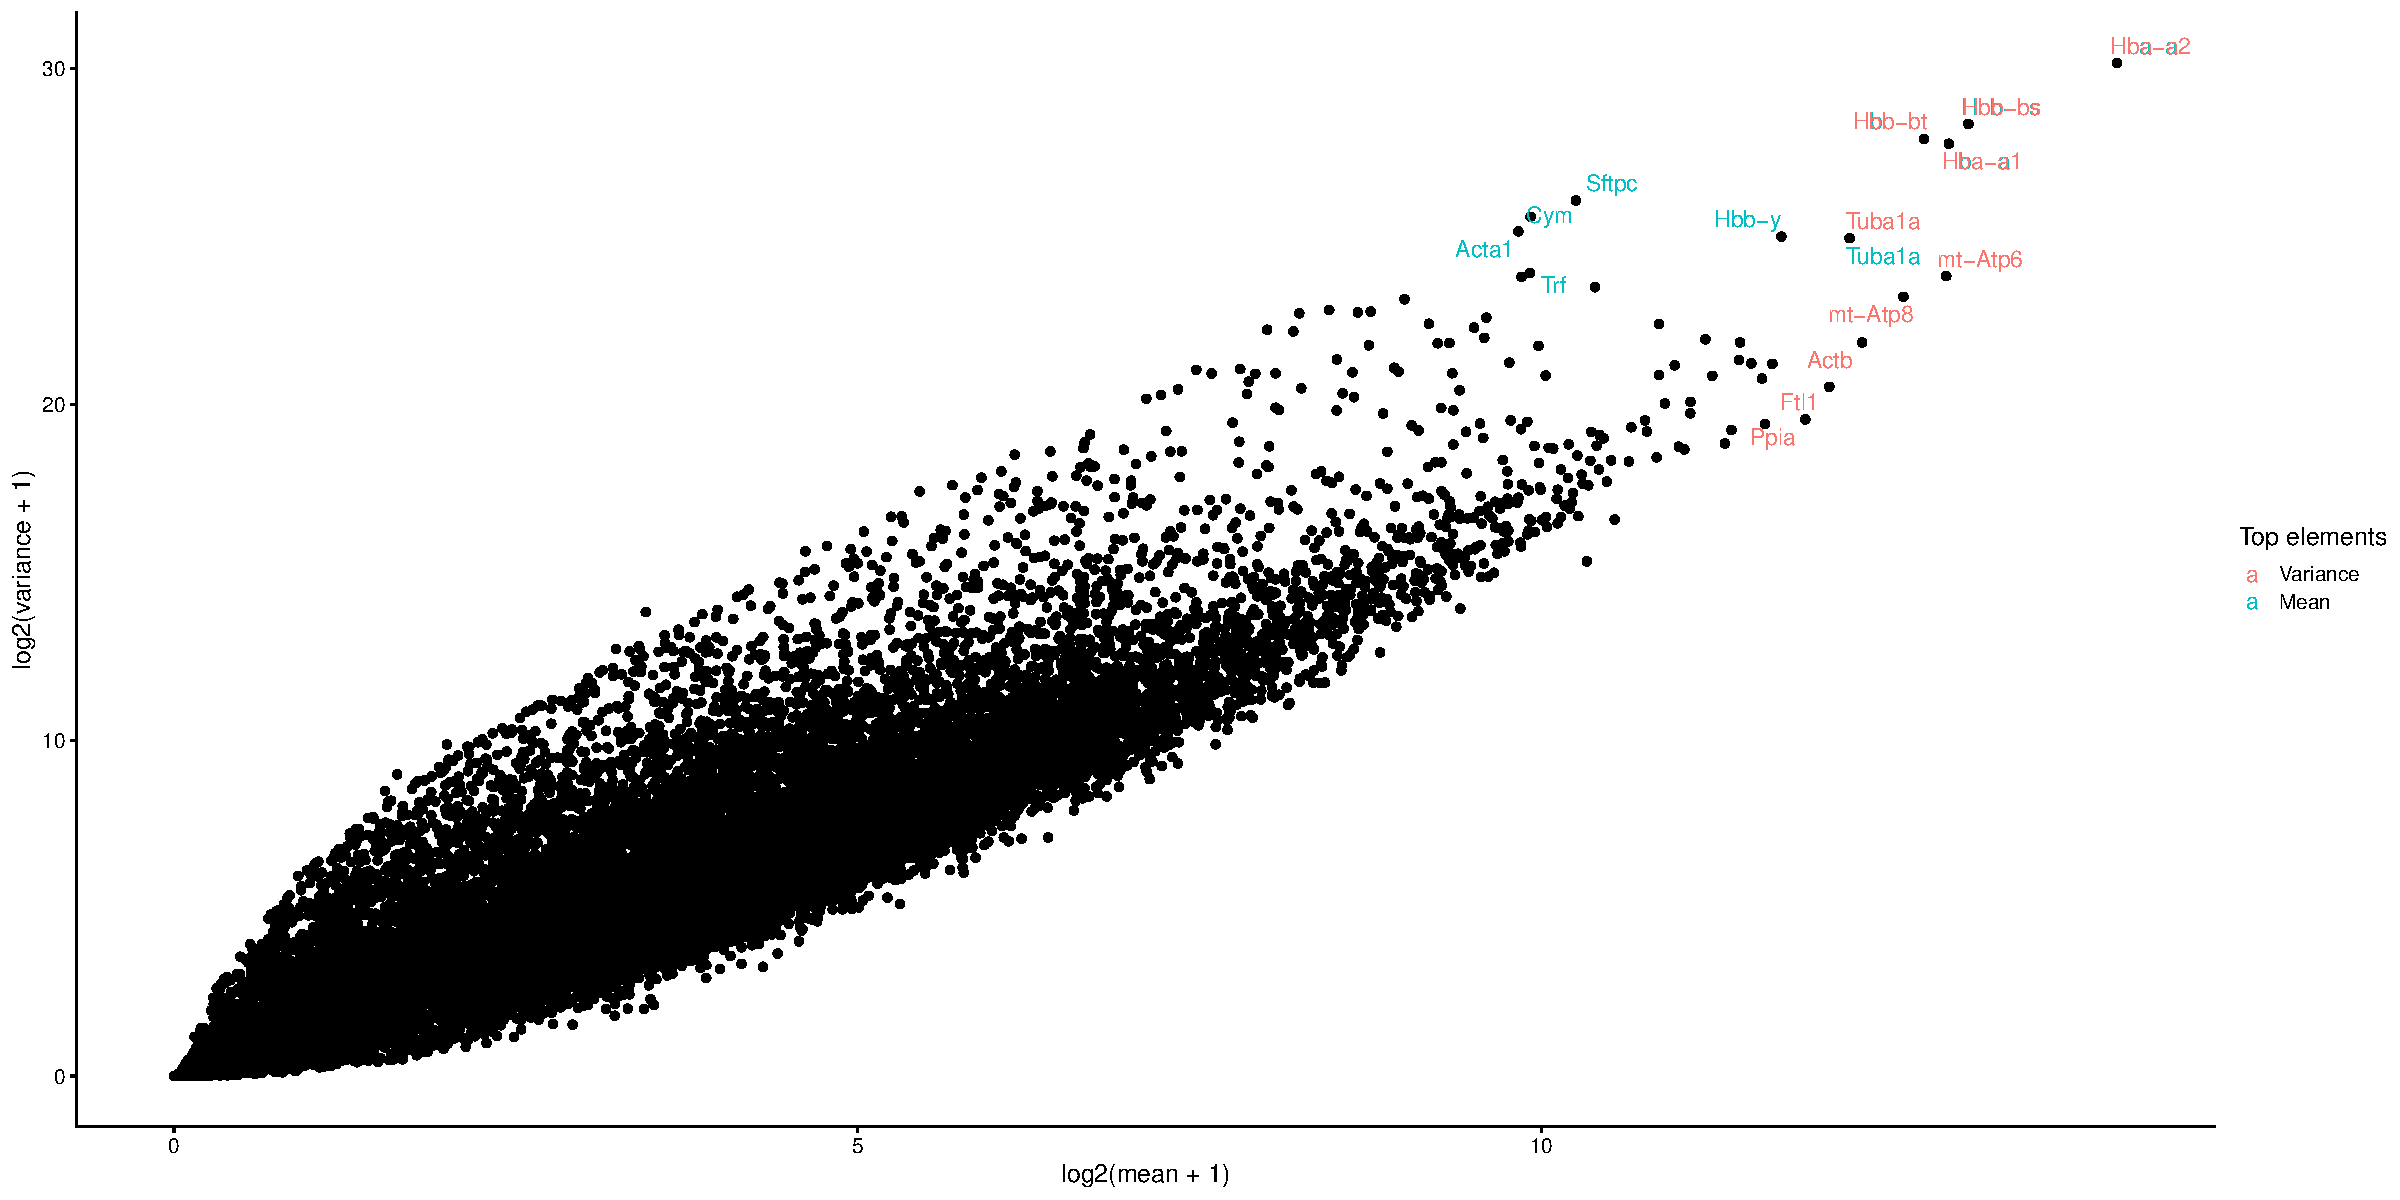
\includegraphics{Exploration_files/figure-latex/unnamed-chunk-15-1.pdf}
Mean and variance all together but hue by organism type

\begin{Shaded}
\begin{Highlighting}[]
\NormalTok{collapsed\_matrices }\OtherTok{\textless{}{-}} \FunctionTok{data.frame}\NormalTok{(}\AttributeTok{mean=}\FunctionTok{double}\NormalTok{(), }\AttributeTok{variance=}\FunctionTok{double}\NormalTok{(), }\AttributeTok{tissue=}\FunctionTok{character}\NormalTok{(), }\AttributeTok{row=}\FunctionTok{character}\NormalTok{())}
\FunctionTok{colnames}\NormalTok{(collapsed\_matrices) }\OtherTok{\textless{}{-}} \FunctionTok{c}\NormalTok{(}\StringTok{"mean"}\NormalTok{, }\StringTok{"variance"}\NormalTok{, }\StringTok{"tissue"}\NormalTok{)}
\ControlFlowTok{for}\NormalTok{ (tissue }\ControlFlowTok{in}\NormalTok{ tissue\_types)\{}
\NormalTok{  tissue\_subset\_ids }\OtherTok{\textless{}{-}}\NormalTok{ meta }\SpecialCharTok{\%\textgreater{}\%} \FunctionTok{filter}\NormalTok{(tissue\_type }\SpecialCharTok{==}\NormalTok{ tissue) }\SpecialCharTok{\%\textgreater{}\%} \FunctionTok{pull}\NormalTok{(id)}
\NormalTok{  all\_means }\OtherTok{\textless{}{-}} \FunctionTok{apply}\NormalTok{(all\_counts[,tissue\_subset\_ids],}\DecValTok{1}\NormalTok{, mean)}
\NormalTok{  all\_variance }\OtherTok{\textless{}{-}} \FunctionTok{apply}\NormalTok{(all\_counts[,tissue\_subset\_ids],}\DecValTok{1}\NormalTok{, var)}
\NormalTok{  temp\_matrix }\OtherTok{\textless{}{-}} \FunctionTok{data.frame}\NormalTok{(}\AttributeTok{mean=}\NormalTok{all\_means, }\AttributeTok{variance=}\NormalTok{all\_variance, tissue) }\SpecialCharTok{\%\textgreater{}\%} \FunctionTok{rownames\_to\_column}\NormalTok{(}\StringTok{"rowname"}\NormalTok{)}
\NormalTok{  collapsed\_matrices }\OtherTok{\textless{}{-}} \FunctionTok{rbind}\NormalTok{(collapsed\_matrices, temp\_matrix)}
\NormalTok{\}}
\FunctionTok{ggplot}\NormalTok{(}\AttributeTok{data=}\NormalTok{collapsed\_matrices, }\FunctionTok{aes}\NormalTok{(}\AttributeTok{x=}\FunctionTok{log2}\NormalTok{(mean}\SpecialCharTok{+}\DecValTok{1}\NormalTok{), }\AttributeTok{y=}\FunctionTok{log2}\NormalTok{(variance}\SpecialCharTok{+}\DecValTok{1}\NormalTok{), }\AttributeTok{colour=}\NormalTok{tissue)) }\SpecialCharTok{+} \FunctionTok{geom\_point}\NormalTok{()}\SpecialCharTok{+} \FunctionTok{theme\_cowplot}\NormalTok{(}\DecValTok{12}\NormalTok{) }\SpecialCharTok{+} 
  \FunctionTok{geom\_text\_repel}\NormalTok{(}\AttributeTok{data=}\NormalTok{collapsed\_matrices }\SpecialCharTok{\%\textgreater{}\%} \FunctionTok{slice\_max}\NormalTok{(variance}\SpecialCharTok{+}\NormalTok{mean, }\AttributeTok{n=}\DecValTok{15}\NormalTok{), }\FunctionTok{aes}\NormalTok{(}\AttributeTok{x=}\FunctionTok{log2}\NormalTok{(mean}\SpecialCharTok{+}\DecValTok{1}\NormalTok{), }\AttributeTok{y=}\FunctionTok{log2}\NormalTok{(variance}\SpecialCharTok{+}\DecValTok{1}\NormalTok{), }\AttributeTok{label=}\NormalTok{rowname, }\AttributeTok{colour=}\NormalTok{tissue)) }
\end{Highlighting}
\end{Shaded}

\includegraphics{Exploration_files/figure-latex/unnamed-chunk-16-1.pdf}

\begin{Shaded}
\begin{Highlighting}[]
  \CommentTok{\#geom\_text\_repel(data=collapsed\_matrices \%\textgreater{}\% rownames\_to\_column("row") \%\textgreater{}\% slice\_max(mean, n=10), aes(x=log2(mean+1), y=log2(variance+1), label=row, colour=tissue))}
  
  \CommentTok{\#scale\_colour\_discrete(name = "Top elements", labels = c("Variance", "Mean"))}
\end{Highlighting}
\end{Shaded}

Variability across tissue types

\begin{Shaded}
\begin{Highlighting}[]
\FunctionTok{ggplot}\NormalTok{(}\AttributeTok{data=}\NormalTok{collapsed\_matrices, }\FunctionTok{aes}\NormalTok{(}\AttributeTok{x=}\FunctionTok{log2}\NormalTok{(mean}\SpecialCharTok{+}\DecValTok{1}\NormalTok{), }\AttributeTok{y=}\FunctionTok{log2}\NormalTok{(variance}\SpecialCharTok{+}\DecValTok{1}\NormalTok{))) }\SpecialCharTok{+} \FunctionTok{geom\_point}\NormalTok{() }\SpecialCharTok{+}  \FunctionTok{facet\_wrap}\NormalTok{(}\SpecialCharTok{\textasciitilde{}}\NormalTok{ tissue, }\AttributeTok{ncol=}\DecValTok{3}\NormalTok{) }\SpecialCharTok{+} \FunctionTok{theme\_cowplot}\NormalTok{(}\DecValTok{12}\NormalTok{) }
\end{Highlighting}
\end{Shaded}

\includegraphics{Exploration_files/figure-latex/unnamed-chunk-17-1.pdf}
Zooming in on highly epxressed gene (\textgreater1025)

\begin{Shaded}
\begin{Highlighting}[]
\FunctionTok{ggplot}\NormalTok{(}\AttributeTok{data=}\NormalTok{collapsed\_matrices  }\SpecialCharTok{\%\textgreater{}\%} \FunctionTok{filter}\NormalTok{(}\FunctionTok{log2}\NormalTok{(mean}\SpecialCharTok{+}\DecValTok{1}\NormalTok{) }\SpecialCharTok{\textgreater{}=}\DecValTok{10}\NormalTok{), }\FunctionTok{aes}\NormalTok{(}\AttributeTok{x=}\FunctionTok{log2}\NormalTok{(mean}\SpecialCharTok{+}\DecValTok{1}\NormalTok{), }\AttributeTok{y=}\FunctionTok{log2}\NormalTok{(variance}\SpecialCharTok{+}\DecValTok{1}\NormalTok{))) }\SpecialCharTok{+} \FunctionTok{geom\_point}\NormalTok{() }\SpecialCharTok{+}  \FunctionTok{facet\_wrap}\NormalTok{(}\SpecialCharTok{\textasciitilde{}}\NormalTok{ tissue, }\AttributeTok{ncol=}\DecValTok{3}\NormalTok{) }\SpecialCharTok{+} \FunctionTok{theme\_cowplot}\NormalTok{(}\DecValTok{12}\NormalTok{) }
\end{Highlighting}
\end{Shaded}

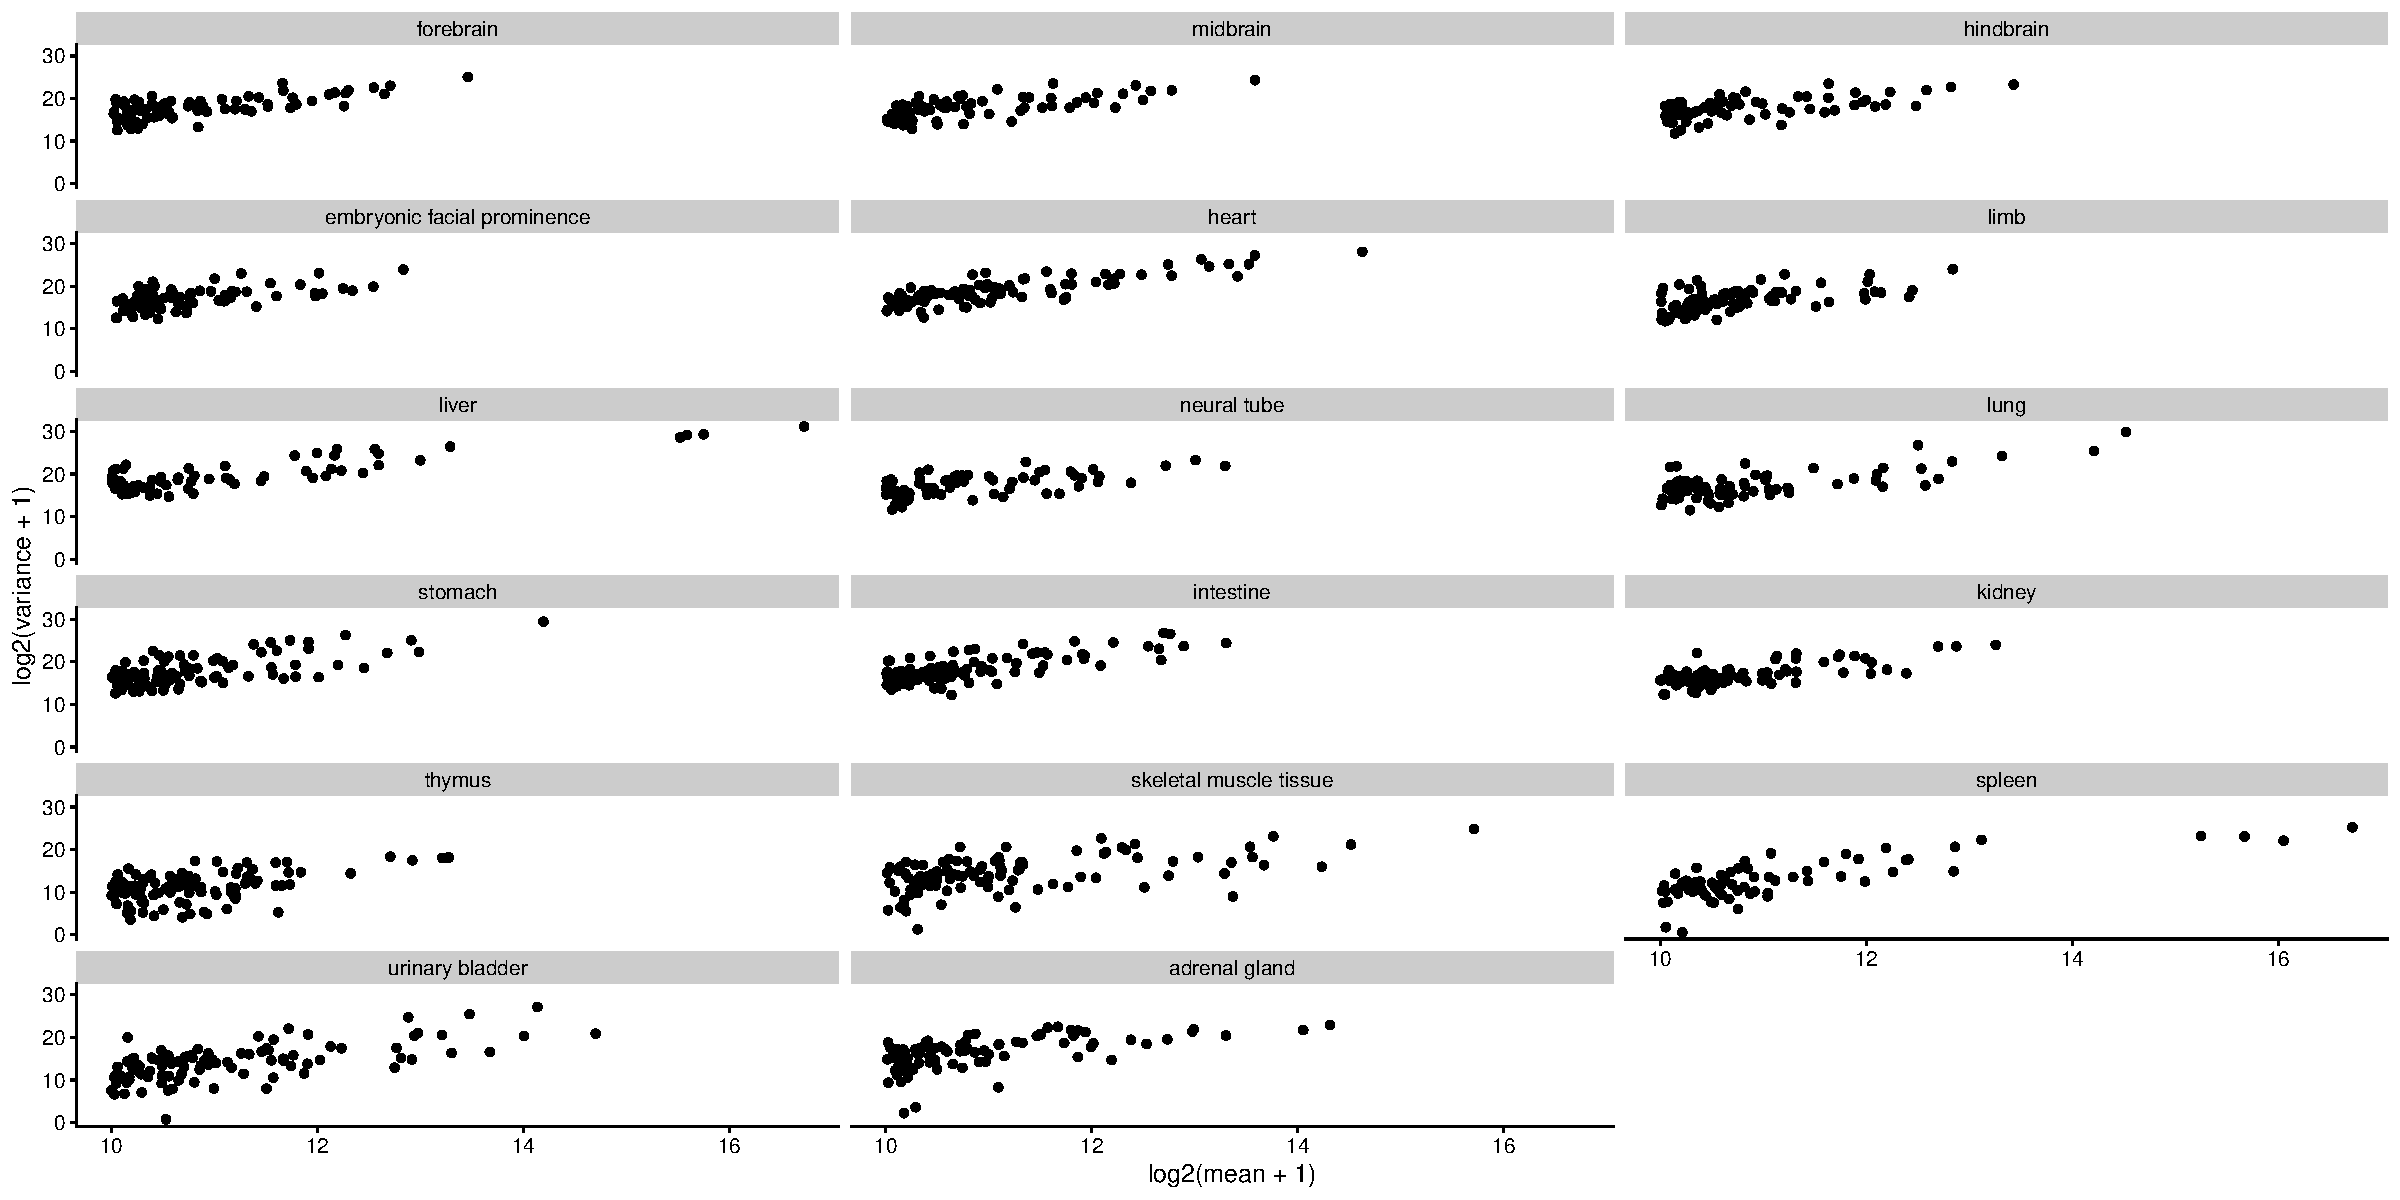
\includegraphics{Exploration_files/figure-latex/unnamed-chunk-18-1.pdf}
Distribution of the TFs

\begin{Shaded}
\begin{Highlighting}[]
\NormalTok{TFCounts }\OtherTok{\textless{}{-}} \FunctionTok{data.frame}\NormalTok{(all\_counts[TFs,])}
\NormalTok{TFCounts }\OtherTok{\textless{}{-}}\NormalTok{ TFCounts }\SpecialCharTok{\%\textgreater{}\%} \FunctionTok{rownames\_to\_column}\NormalTok{(}\StringTok{"rowname"}\NormalTok{)}
\NormalTok{TFCounts }\OtherTok{\textless{}{-}}\NormalTok{ TFCounts }\SpecialCharTok{\%\textgreater{}\%} \FunctionTok{gather}\NormalTok{(}\StringTok{"id"}\NormalTok{, }\StringTok{"counts"}\NormalTok{, }\SpecialCharTok{{-}}\NormalTok{rowname)}
\NormalTok{TFCounts }\OtherTok{\textless{}{-}}\NormalTok{ TFCounts }\SpecialCharTok{\%\textgreater{}\%} \FunctionTok{left\_join}\NormalTok{((meta }\SpecialCharTok{\%\textgreater{}\%} \FunctionTok{select}\NormalTok{(tissue\_type, dev\_stage, id)), }\AttributeTok{by=}\StringTok{"id"}\NormalTok{)}

\FunctionTok{ggplot}\NormalTok{(}\AttributeTok{data=}\NormalTok{TFCounts, }\FunctionTok{aes}\NormalTok{(}\AttributeTok{x=}\NormalTok{counts)) }\SpecialCharTok{+} \FunctionTok{geom\_histogram}\NormalTok{(}\AttributeTok{bins =} \DecValTok{100}\NormalTok{) }\SpecialCharTok{+} \FunctionTok{facet\_grid}\NormalTok{(}\SpecialCharTok{\textasciitilde{}}\NormalTok{  rowname) }\SpecialCharTok{+} \FunctionTok{theme\_cowplot}\NormalTok{(}\DecValTok{12}\NormalTok{)}
\end{Highlighting}
\end{Shaded}

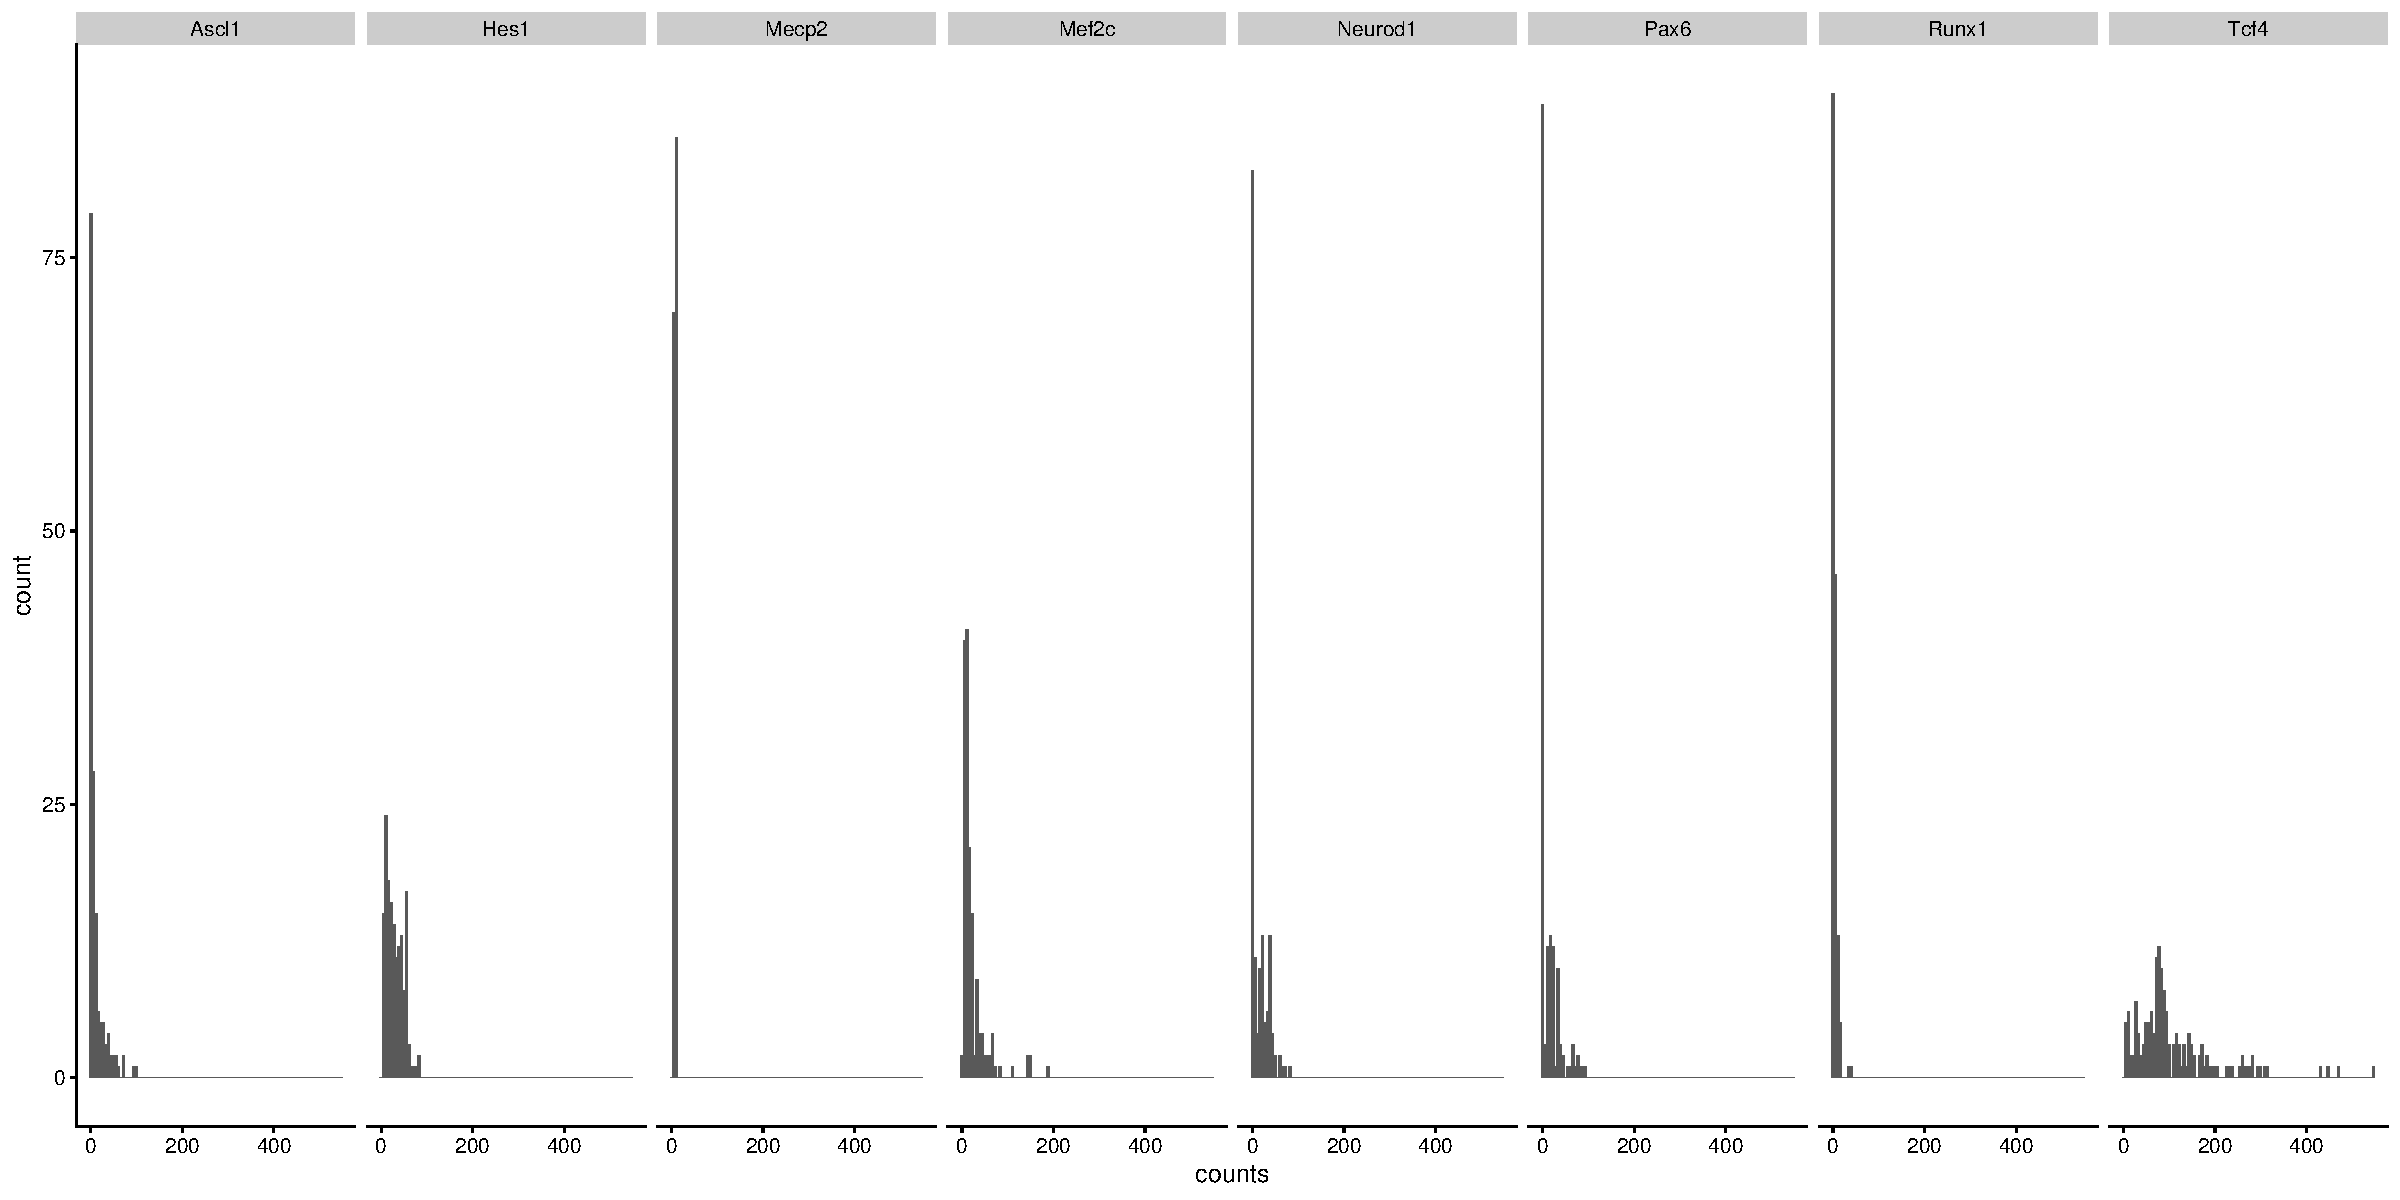
\includegraphics{Exploration_files/figure-latex/unnamed-chunk-19-1.pdf}
Distribution of the TFs (Log transformed)

\begin{Shaded}
\begin{Highlighting}[]
\NormalTok{TFCounts }\OtherTok{\textless{}{-}} \FunctionTok{data.frame}\NormalTok{(all\_counts[TFs,])}
\NormalTok{TFCounts }\OtherTok{\textless{}{-}}\NormalTok{ TFCounts }\SpecialCharTok{\%\textgreater{}\%} \FunctionTok{rownames\_to\_column}\NormalTok{(}\StringTok{"rowname"}\NormalTok{)}
\NormalTok{TFCounts }\OtherTok{\textless{}{-}}\NormalTok{ TFCounts }\SpecialCharTok{\%\textgreater{}\%} \FunctionTok{gather}\NormalTok{(}\StringTok{"id"}\NormalTok{, }\StringTok{"counts"}\NormalTok{, }\SpecialCharTok{{-}}\NormalTok{rowname)}
\NormalTok{TFCounts }\OtherTok{\textless{}{-}}\NormalTok{ TFCounts }\SpecialCharTok{\%\textgreater{}\%} \FunctionTok{left\_join}\NormalTok{((meta }\SpecialCharTok{\%\textgreater{}\%} \FunctionTok{select}\NormalTok{(tissue\_type, dev\_stage, id)), }\AttributeTok{by=}\StringTok{"id"}\NormalTok{)}

\FunctionTok{ggplot}\NormalTok{(}\AttributeTok{data=}\NormalTok{TFCounts, }\FunctionTok{aes}\NormalTok{(}\AttributeTok{x=}\FunctionTok{log2}\NormalTok{(counts}\SpecialCharTok{+}\DecValTok{1}\NormalTok{))) }\SpecialCharTok{+} \FunctionTok{geom\_histogram}\NormalTok{(}\AttributeTok{bins =} \DecValTok{100}\NormalTok{) }\SpecialCharTok{+} \FunctionTok{facet\_grid}\NormalTok{(}\SpecialCharTok{\textasciitilde{}}\NormalTok{  rowname) }\SpecialCharTok{+} \FunctionTok{theme\_cowplot}\NormalTok{(}\DecValTok{12}\NormalTok{)}
\end{Highlighting}
\end{Shaded}

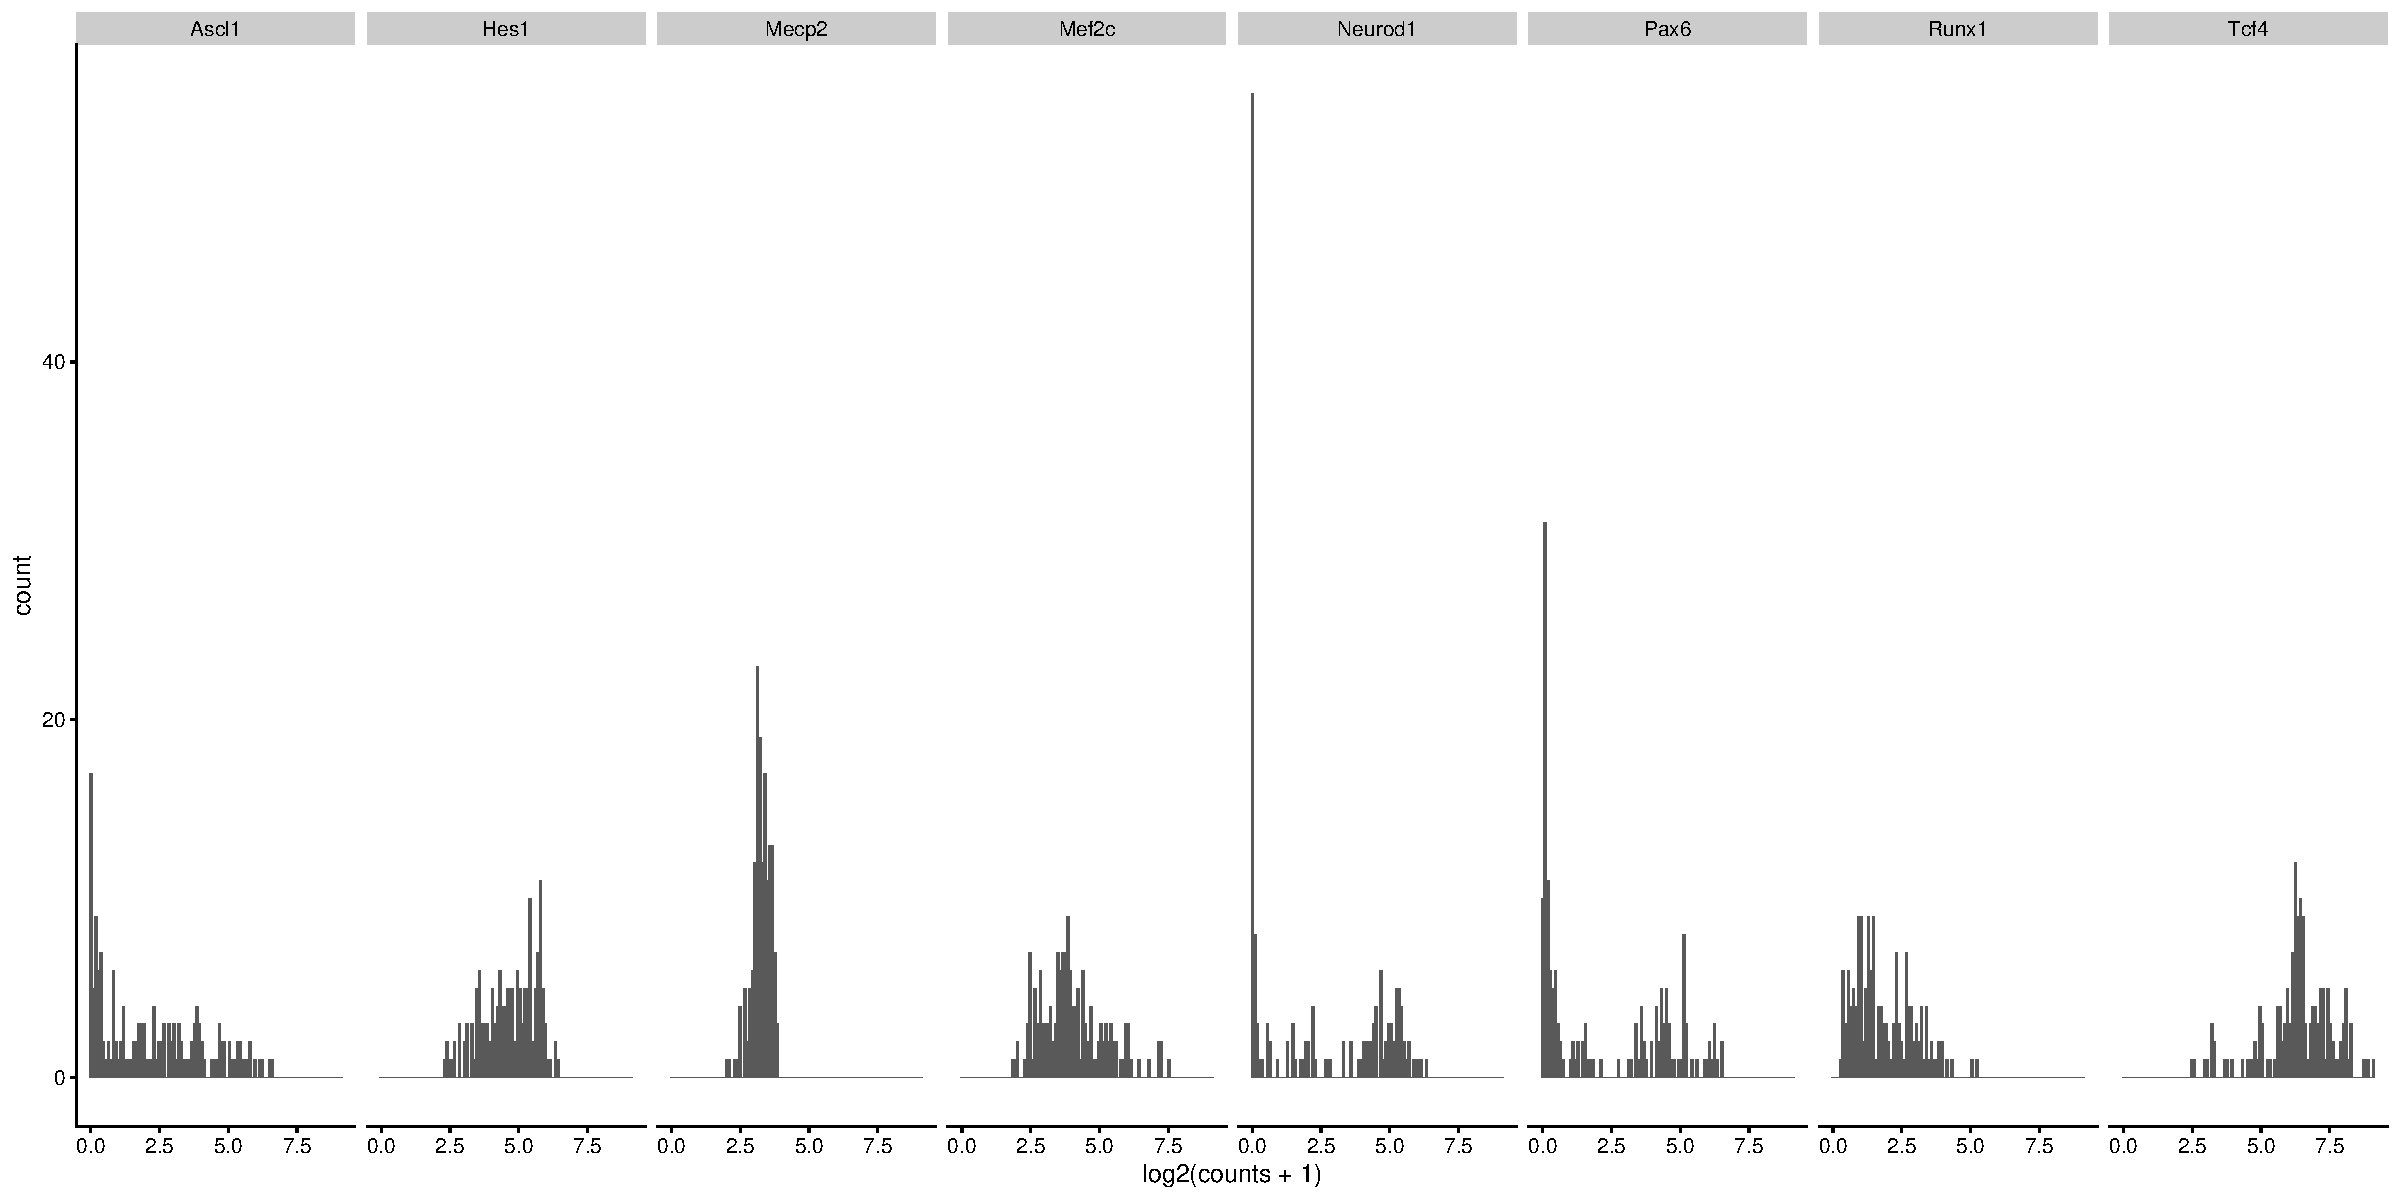
\includegraphics{Exploration_files/figure-latex/unnamed-chunk-20-1.pdf}
Distribution of the TFs (Log transformed)

\begin{Shaded}
\begin{Highlighting}[]
\NormalTok{TFCounts }\OtherTok{\textless{}{-}} \FunctionTok{data.frame}\NormalTok{(all\_counts[TFs,])}
\NormalTok{TFCounts }\OtherTok{\textless{}{-}}\NormalTok{ TFCounts }\SpecialCharTok{\%\textgreater{}\%} \FunctionTok{rownames\_to\_column}\NormalTok{(}\StringTok{"rowname"}\NormalTok{)}
\NormalTok{TFCounts }\OtherTok{\textless{}{-}}\NormalTok{ TFCounts }\SpecialCharTok{\%\textgreater{}\%} \FunctionTok{gather}\NormalTok{(}\StringTok{"id"}\NormalTok{, }\StringTok{"counts"}\NormalTok{, }\SpecialCharTok{{-}}\NormalTok{rowname)}
\NormalTok{TFCounts }\OtherTok{\textless{}{-}}\NormalTok{ TFCounts }\SpecialCharTok{\%\textgreater{}\%} \FunctionTok{left\_join}\NormalTok{((meta }\SpecialCharTok{\%\textgreater{}\%} \FunctionTok{select}\NormalTok{(tissue\_type, dev\_stage, id)), }\AttributeTok{by=}\StringTok{"id"}\NormalTok{)}

\FunctionTok{ggplot}\NormalTok{(}\AttributeTok{data=}\NormalTok{collapsed\_matrices }\SpecialCharTok{\%\textgreater{}\%} \FunctionTok{filter}\NormalTok{(rowname }\SpecialCharTok{\%in\%}\NormalTok{ TFs), }\FunctionTok{aes}\NormalTok{(}\AttributeTok{x=}\FunctionTok{log2}\NormalTok{(mean}\SpecialCharTok{+}\DecValTok{1}\NormalTok{), }\AttributeTok{y=}\FunctionTok{log2}\NormalTok{(variance}\SpecialCharTok{+}\DecValTok{1}\NormalTok{), }\AttributeTok{colour=}\NormalTok{tissue)) }\SpecialCharTok{+} \FunctionTok{geom\_point}\NormalTok{()}\SpecialCharTok{+} \FunctionTok{theme\_cowplot}\NormalTok{(}\DecValTok{12}\NormalTok{) }\SpecialCharTok{+} 
  \FunctionTok{geom\_text\_repel}\NormalTok{(}\AttributeTok{data=}\NormalTok{collapsed\_matrices }\SpecialCharTok{\%\textgreater{}\%} \FunctionTok{filter}\NormalTok{(rowname }\SpecialCharTok{\%in\%}\NormalTok{ TFs) }\SpecialCharTok{\%\textgreater{}\%} \FunctionTok{slice\_max}\NormalTok{(variance}\SpecialCharTok{+}\NormalTok{mean, }\AttributeTok{n=}\DecValTok{15}\NormalTok{), }\FunctionTok{aes}\NormalTok{(}\AttributeTok{x=}\FunctionTok{log2}\NormalTok{(mean}\SpecialCharTok{+}\DecValTok{1}\NormalTok{), }\AttributeTok{y=}\FunctionTok{log2}\NormalTok{(variance}\SpecialCharTok{+}\DecValTok{1}\NormalTok{), }\AttributeTok{label=}\NormalTok{rowname, }\AttributeTok{colour=}\NormalTok{tissue)) }
\end{Highlighting}
\end{Shaded}

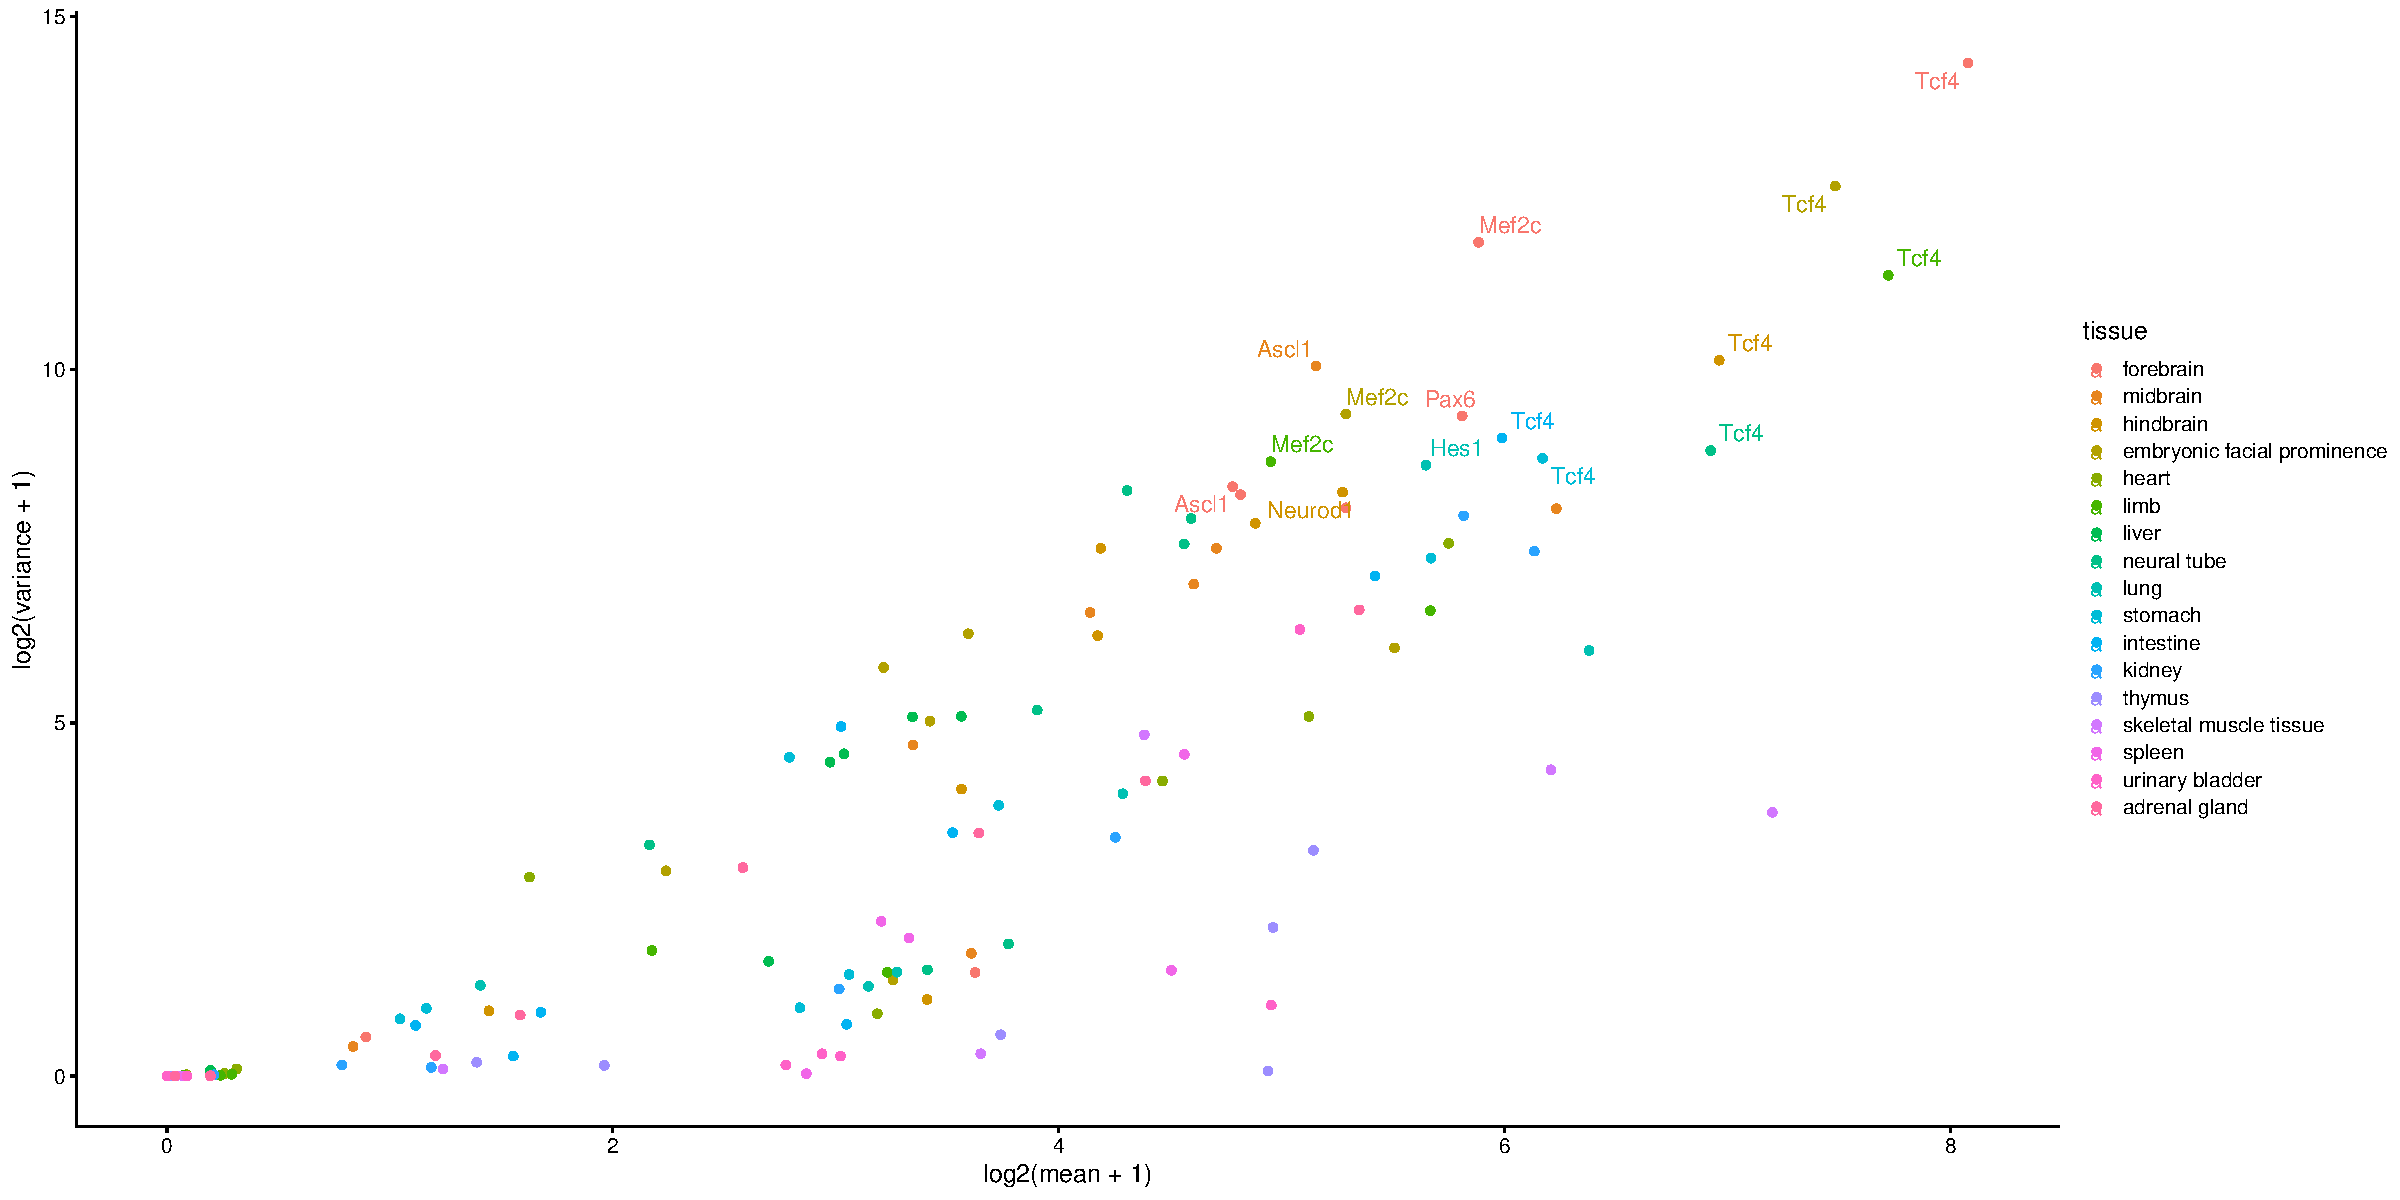
\includegraphics{Exploration_files/figure-latex/unnamed-chunk-21-1.pdf}

look at 10 genese Completely different expression pattern in different
tissues

variability (across tissues, within tissues as well) mean-variance is
the ranking similar across tissues

\begin{Shaded}
\begin{Highlighting}[]
\DocumentationTok{\#\#Remove zero variance }
\NormalTok{all\_counts\_drop\_var }\OtherTok{\textless{}{-}}\NormalTok{ (}\FunctionTok{t}\NormalTok{(all\_counts))[, }\FunctionTok{which}\NormalTok{(}\FunctionTok{apply}\NormalTok{(}\FunctionTok{t}\NormalTok{(all\_counts),}\DecValTok{2}\NormalTok{,var) }\SpecialCharTok{!=}\DecValTok{0}\NormalTok{)]}
\NormalTok{all\_counts.pca }\OtherTok{\textless{}{-}} \FunctionTok{prcomp}\NormalTok{(all\_counts\_drop\_var, }\AttributeTok{center =} \ConstantTok{TRUE}\NormalTok{,}\AttributeTok{scale. =} \ConstantTok{TRUE}\NormalTok{)}
\FunctionTok{library}\NormalTok{(ggfortify)}
\FunctionTok{autoplot}\NormalTok{(all\_counts.pca, }\AttributeTok{data=}\NormalTok{meta, }\AttributeTok{colour=}\StringTok{"dev\_stage"}\NormalTok{) }\SpecialCharTok{+} \FunctionTok{theme\_cowplot}\NormalTok{(}\DecValTok{12}\NormalTok{)}
\end{Highlighting}
\end{Shaded}

\includegraphics{Exploration_files/figure-latex/unnamed-chunk-22-1.pdf}

\end{document}
